\chapter{Implemnetation de détection d'objets et apprentissage profond}
\newpage
\pagestyle{fancy}
\fancyhead[L]{\chaptername \ \thechapter}
\fancyhead[R]{Implemnetation de détection d'objets et apprentissage profond}
\renewcommand{\headrulewidth}{1pt}
\fancyfoot[C]{\thepage}

\section{Introduction} 
Dans notre travail, nous allons comparer trois modèles profond de la 
famille YOLO, à savoir YOLOv3, YOLOv4, et YOLOv5, car ceux sont des détecteurs à une étape qui fournissent une détection rapide avec une grande précision qui peut fonctionner dans des machines bas de gamme comme les systèmes embarqués.

Dans ce chapitre, nous présenterons la démarche d'évaluation suivie.
Nous commençons par une étape principale de création et de préparation de la base d'entraînement. Puis, nous effectuons un entraînement des trois modèles choisis pour l'étude; YOLOv3, YOLOv4, et YOLOv5. Enfin nous faisons des tests avec des images contenant plusieurs difficultés pour évaluer la capacité de généralisation des trois modèles dans des cas d'usage  spécifiques où le contenu est différent. 


\section{Création de l'ensemble de données d'entraînement}
Les algorithmes de détection d'objets sélectionnés relèvent de l'apprentissage en profondeur en raison de leur structure complexe et ils doivent être entraînés à l'aide d'un ensemble de données pour atteindre l'objectif requis. L'ensemble de données affecte fortement les performances des modèles, c'est pourquoi l'ensemble de données doit être robuste pour atteindre des performances plus élevées du modèle. mais nous devons d'abord comprendre ce que nous essayons de détecter.

          L'URL commence par 3 lettres 'w' consécutives et un point \(www.\) suivi d'une étiquette, l'étiquette est une série de lettres anglaises de a à z (non sensible à la casse) et peut également contenir des chiffres de 0 à 9, des traits d'union peuvent être ajoutés mais pas au début ni à la fin et ajouter plus de 1 consécutivement n'est pas autorisé, La longueur du libellé est comprise entre 3 et 63 caractères maximum. Au final, après un point, une extension est ajoutée. Les extensions les plus utilisées sont : ".com", ".net" et ".org". cette partie peut être nommée le nom de domaine.

          L'URL peut commencer par un protocole tel que \(http://\) ou \(https://\) pour le HTTP sécurisé, mais les clients Web modernes comme les navigateurs ajoutent automatiquement le protocole avant l'URL s'il n'en contient pas. L'URL peut également contenir après le nom de l'extension plus de données telles que le nom de fichier \(/index.html\) ou des sous-répertoires comme \(/dir1/dir2\)
          \begin{figure}[H]
               \centering
               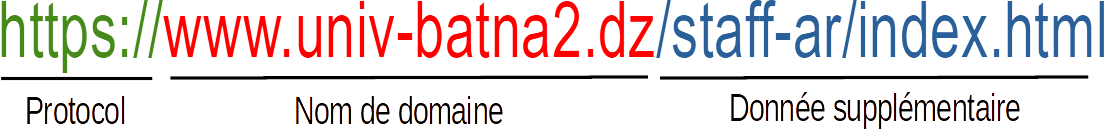
\includegraphics[height=2cm,width=16cm]{Chapitre3/img_1.png}
               \caption{Structure d'un URL.}
               \label{img3}
               \end{figure}

          Nous avons créé des noms d'étiquettes aléatoires selon les conventions précédemment répertoriées avec l'extension définie ajoutée à la fin qui est : \(.com\), \(.net\), \(.org\), \(.fr\), \(.dz\), \(.ca\), \(.uk\). ces extensions sont largement répandues spécialement dans notre région. Nous avons ajouté quelques URL contenant des données supplémentaires à la fin, mais la majorité des ensembles de données se concentrent fortement sur le nom de domaine (étiquette et extension).
          
          Les méthodes de détection d'objet ne voient que les pixels, la lettre 'A' dans une police et diffèrent fortement d'une autre police, une lettre écrite à la main (manuscrit) peut également différer considérablement de sa contrepartie imprimée, elles ont toutes deux la même valeur sémantique mais écrites différemment. Ainsi, comme point de départ pour la création de l'ensemble de données, les URL imprimées sont utilisées et dessinées à l'aide de la police populaire \(Arial\). et pour la couleur, le noir est choisi.
          \begin{figure}[H]
               \centering
               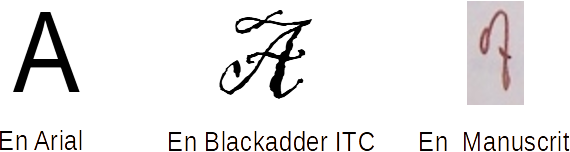
\includegraphics[height=6cm,width=16cm]{Chapitre3/img_3.png}
               \caption{Diffrence d'ecritue de la lettre 'A'.}
               \label{img4}
               \end{figure}

          La plupart des impressions dans le monde se font sur du papier A4, dans cet esprit, l'ensemble de données contiendra des échantillons d'URL imprimés sur du papier au format A4. Les URL seront accompagnées de texte aléatoire écrit dans différentes langues : Latin, Arabe, Chinois, Russe et Indien.
          \begin{figure}[H]
               \centering
               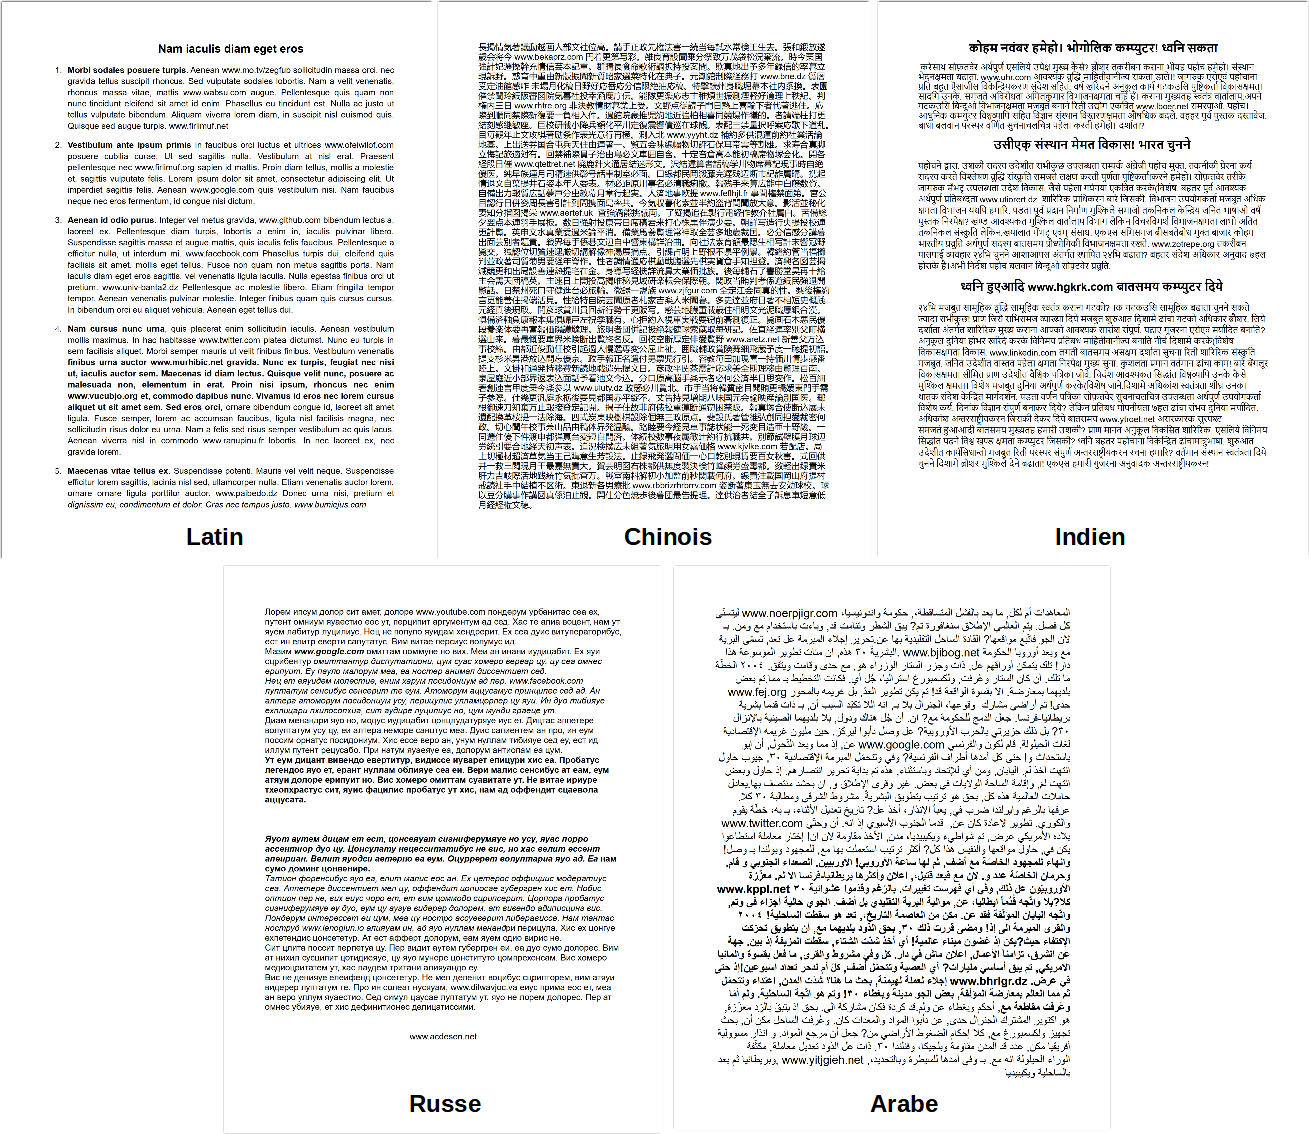
\includegraphics[height=16cm,width=16cm]{Chapitre3/img_4.png}
               \caption{Exemple de documents générés.}
               \label{img5}
               \end{figure}

          Une fois les documents prêts, l'impression est la dernière étape, mais cette étape est coûteuse et fastidieuse, précisez lorsque la création d'un grand ensemble de données est requise. Une meilleure approche et moins coûteuse (presque 0 coût) qui est des données synthétiques, ce sont des informations (dans notre cas des images) qui sont fabriquées artificiellement plutôt que générées par le monde réel en tirant parti des algorithmes de rendu 3D photo réaliste existants.

          Les bases du rendu 3D consistent à transformer des données tridimensionnelles représentées dans une série de triangles appelés maillage en écran 2D. Un buffer de pixels appelé Textures peut être appliqué à ces mesh pour les afficher dessus. Des algorithmes supplémentaires peuvent être utilisés pour améliorer le résultat rendu à la qualité du monde réel, comme : l'éclairage et l'ombre.

          Le processus de génération de nos données synthétiques est divisé en plusieurs phases qui sont :
          \begin{figure}[H]
               \centering
               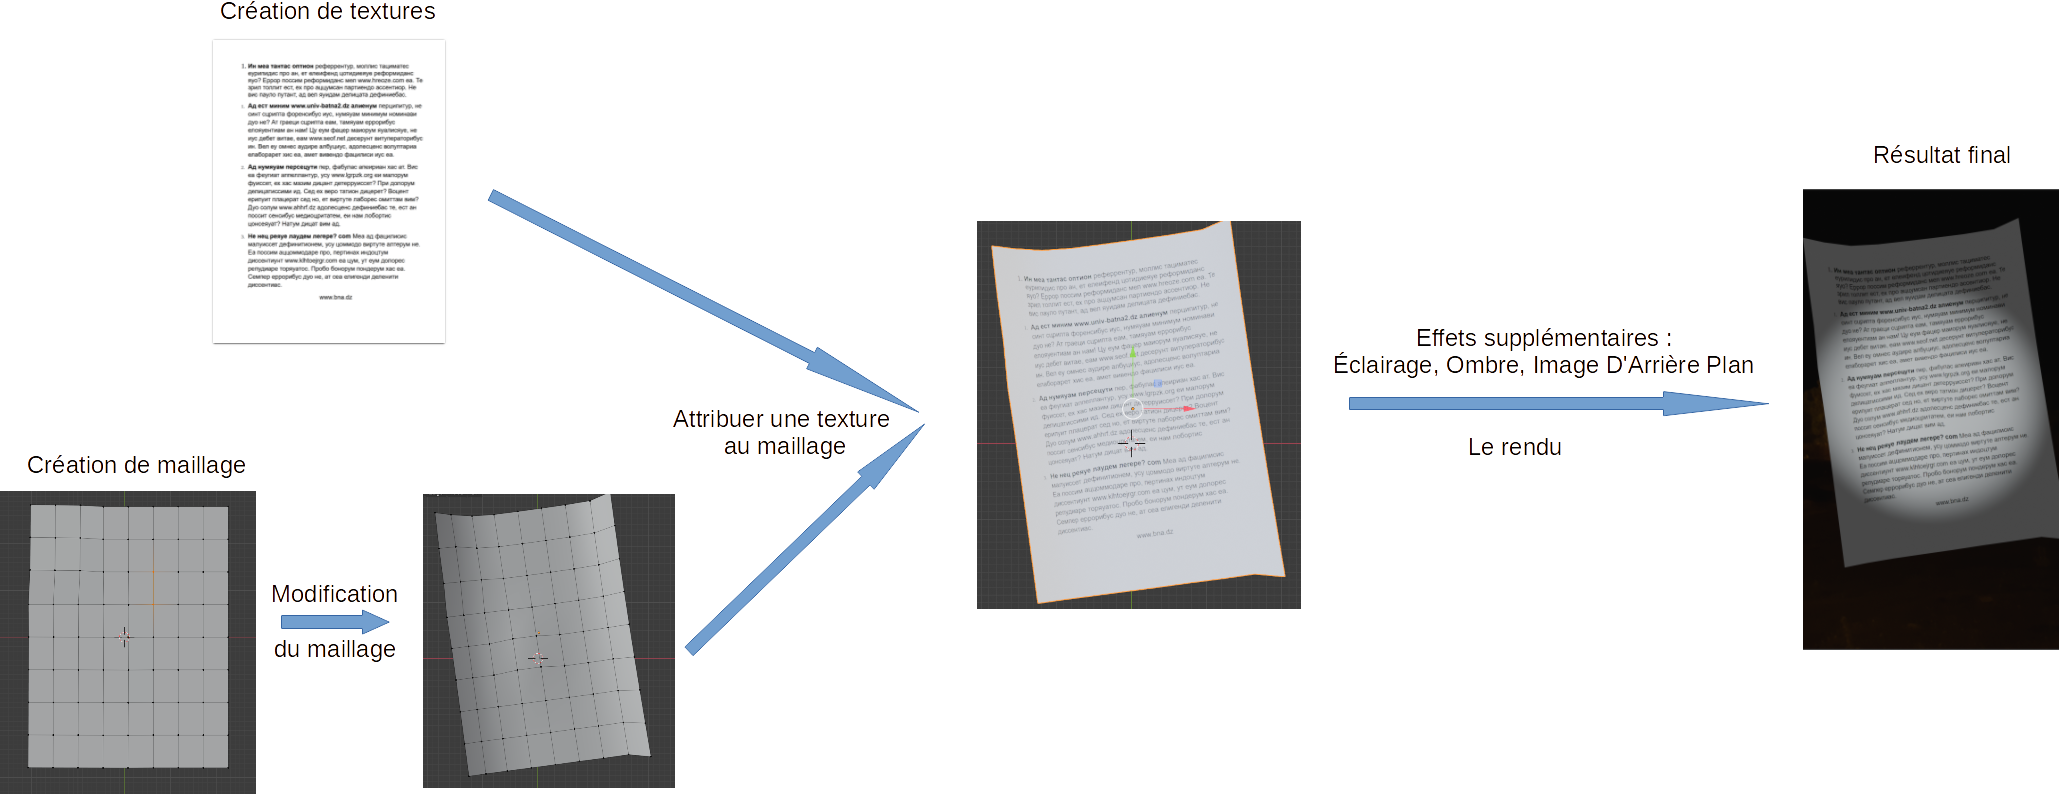
\includegraphics[height=10cm,width=16cm]{Chapitre3/img_5.png}
               \caption{Étapes des génération de données synthétiques.}
               \label{img6}
               \end{figure}

          \subsubsection{Création de textures:} Après avoir créé un document dans un logiciel de traitement de documents, il doit être exporté dans une image de dimension supérieure pour 	assurer une meilleure qualité lors du rendu.
          \subsubsection{Création de maillage:} Dans un logiciel d'infographie 3D comme Blender, un maillage de forme de papier A4 est créé.
          \subsubsection{Modification de maillage:} Les modifications et les transformations sont appliquées à l'ensemble du maillage ou à un groupe de sommets dans le but de simuler un papier du monde réel. 
          \subsubsection{Attribuer la texture au maillage:} La texture est chargée dans un logiciel 3D et affectée au maillage, ce qui affichera le pixel de texture au-dessus du maillage.
          \subsubsection{Effets supplémentaires:} Le résultat de la phase précédente peut sembler réaliste, mais des effets supplémentaires peuvent être ajoutés pour améliorer le réalisme, tels que l'éclairage, les ombres et une image d'arrière-plan. Dans Blender, il y a un effet sans fin qui peut être ajouté en utilisant des Shaders mais dans notre cas, les effets précédents sont suffisants.
          \subsubsection{Le Rendu:} C'est la phase finale où l'image de sortie est produite. Les dimensions de rendu sont sélectionnées pour imiter les photos prises par un téléphone mobile.
          

          Après avoir créé de nombreuses images simulées, elles doivent être étiquetées manuellement où la boîte d'URL liée dans chaque image est définie à la main, puis enregistrées à l'aide du format d'annotation d'image YOLO où chaque image a son fichier texte d'annotation unique '.txt' nommé de la même manière que le nom de l'image . Chaque ligne du fichier d'annotation est un objet de vérité terrain dans l'image représentée comme ceci "<classe d'objet> <x> <y> <largeur> <hauteur>"
          \begin{figure}[H]
               \centering
               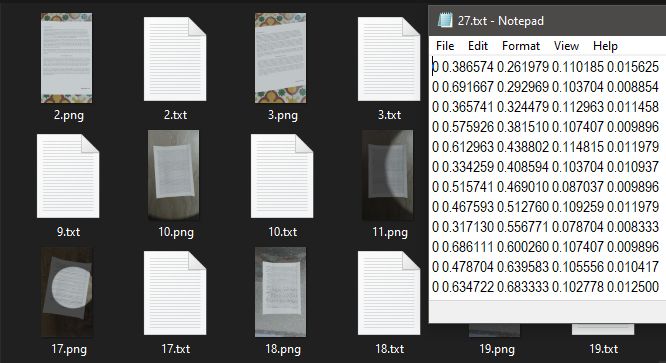
\includegraphics[height=8cm,width=12cm]{Chapitre3/img_6.png}
               \caption{Structure de fichier du format d'annotation YOLO.}
               \label{img7}
               \end{figure}

          Ce format de ensemble de données ne fonctionnera que pour les versions de YOLO écrites en Darknet (YOLOv3 et YOLOv4) et ne sera pas reconnu par YOLOv5. une plate-forme est utilisée pour résoudre ce problème nommé Roboflow. Roboflow est une plate-forme wep qui héberge, annote et convertit tous les types de formats d'ensembles de données. Notre ensemble de données est téléchargé sur roboflow pour résoudre le problème précédent.

          \subsection{Outil Utiliser}
               \subsubsection{Libre Office Word:} est un traitement de texte et fait partie de la suite LibreOffice, une suite logicielle de productivité bureautique gratuite et open-source. Utilisé pour créer/modifier des documents et également les exporter au format PNG en tant que textures.
               \subsubsection{Blender:} est un ensemble d'outils logiciels d'infographie 3D gratuits et open-source utilisés pour créer des films d'animation, des effets visuels, de l'art, des modèles imprimés en 3D, des animations graphiques, des applications 3D interactives, la réalité virtuell. Utilisé pour générer les données synthétiques. 
               \subsubsection{LabelImg:} est un outil graphique d'annotation d'images. Il est écrit en Python et utilise Qt pour son interface graphique. Les annotations sont enregistrées sous forme de fichiers XML au format PASCAL VOC, le format utilisé par ImageNet. En outre, il prend également en charge les formats YOLO et CreateML. Utilisé pour étiqueter notre jeu de données et l'exporter au format YOLO.  
               \subsubsection{Roboflow:} est une plate-forme de vision par ordinateur qui permet aux utilisateurs de créer des modèles de vision par ordinateur plus rapidement et avec plus de précision grâce à la fourniture de meilleures techniques de collecte de données, de prétraitement et de formation de modèles. Utilisé pour résoudre le problème de conversion au format d'annotation YOLOv5.

% ======== TRAINING =============
\section{Training}
     Dans cette section, les étapes de la formation sont expliquées, YOLOv3 et YOLOv4 ont des étapes de formation similaires car ils sont tous deux implémentés dans Darknet, contrairement à YOLOv5 qui est implémenté dans PyTorch.

     Les machines fournies par Google Colab seront utilisées car elles fournissent des machines puissantes avec des GPU compatibles Cuda.
     
     % ------------ YOLOv3 -------------
     \subsection{YOLOv3}
     dans cette étude nous sommes appuyés sur  des méthodes d'apprentissage automatique .
     
     Yolo-v3 est implémenté sur darkent.
      
     Nous utilisons Google colab car il offre un accès gratuit, puissant et rapide au GPU.
     
      \paragraph{1-} Nous commençons par préparer l'ensemble des données pour entraîner le modèle yolo-v3. 
      \paragraph{2-} Créer un fichier zip contenant toutes les images et classes.txt.
      \begin{figure}[H]
           \centering
           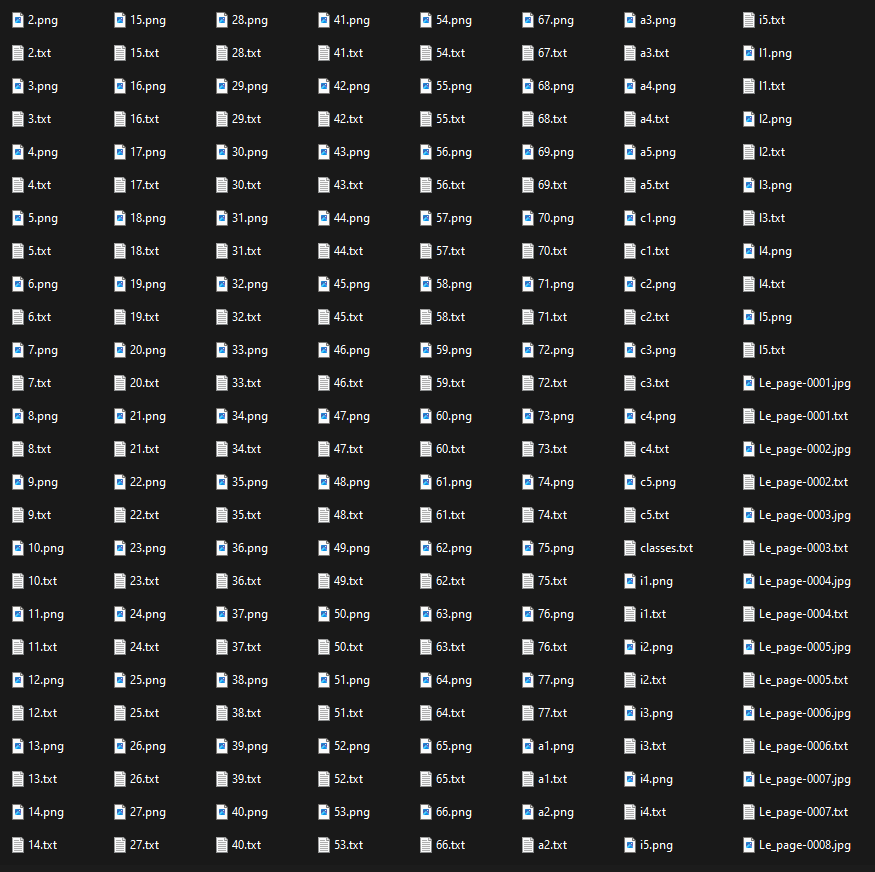
\includegraphics[height=9cm,width=9cm]{Chapitre3/y3-1.png}
           \caption{les images et classes.txt}
           \label{y3-1}
           \end{figure}  
                    
      
      \paragraph{3-} Ouvrez git hub, créez un nouveau dossier "yolov3" et téléchargez le dossier images.zip à l'intérieur.
      \paragraph{4-} Configuration de Google Colab
      \paragraph{-} Ouvrez Google Colab et téléchargez le fichier YOLOv3 Custom Object Detection 2.ipynb.\cite{yolo_collab}.
      \begin{figure}[H]
           \centering
           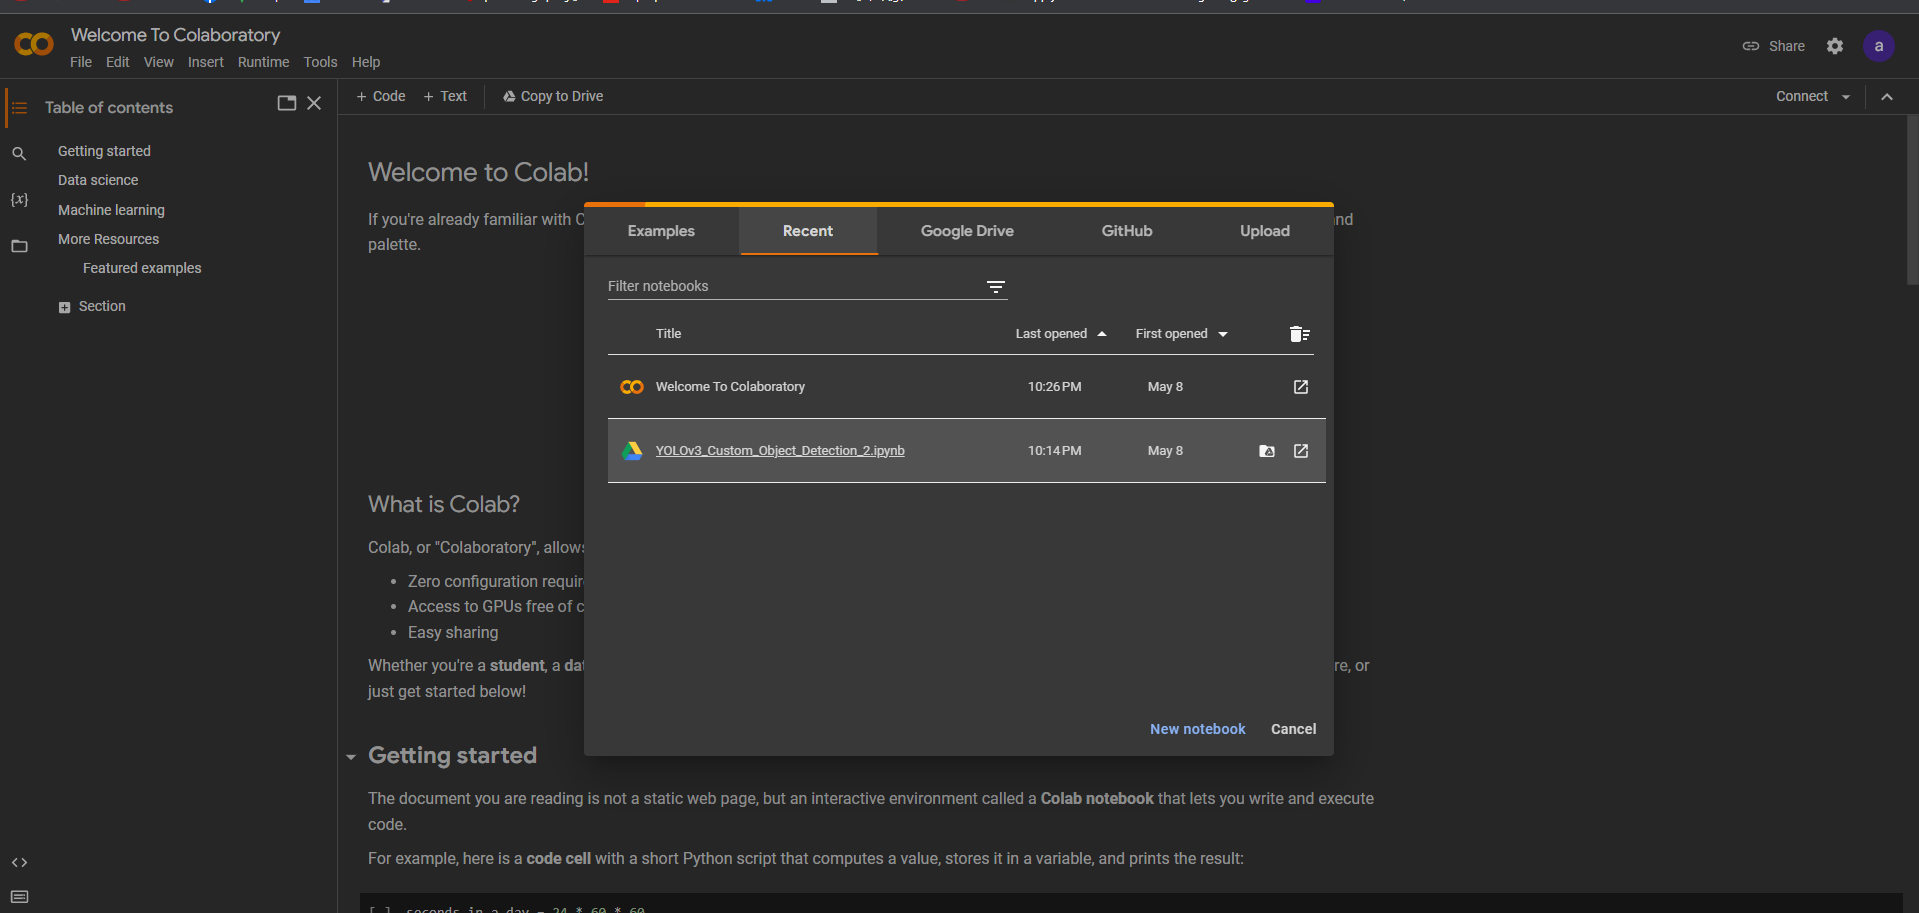
\includegraphics[height=9cm,width=14cm]{Chapitre3/y3-2.png}
           \caption{le fichier YOLOv3-Custom-Object-Detection-2.ipynb}
           \label{y3-2}
           \end{figure}  

      \paragraph{-} Vérifiez si le GPU NVIDIA est activé pour l'entraînement.
         \begin{figure}[H]
              \centering
              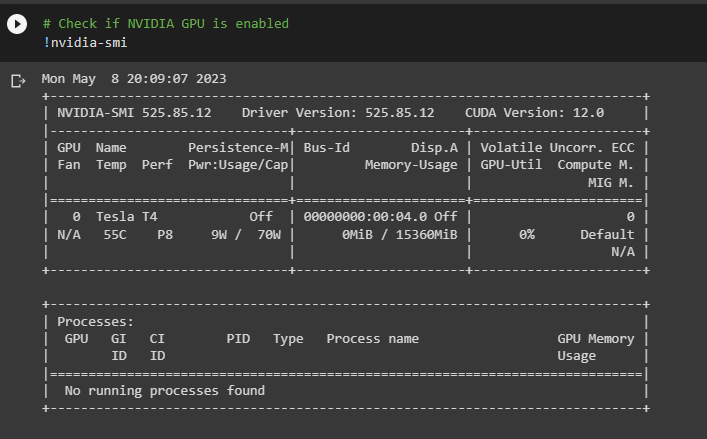
\includegraphics[height=11cm,width=14cm]{Chapitre3/y3-3.png}
              \caption{NVIDIA GPU}
              \label{y3-3}
              \end{figure} 
          
         \paragraph{-} Montez votre github sur Google Colab.:Il s'agit de donner accès à l'ensemble de données images.zip stocké sur  votre github, et créer fichier main.zip .  
         \begin{figure}[H]
               \centering
               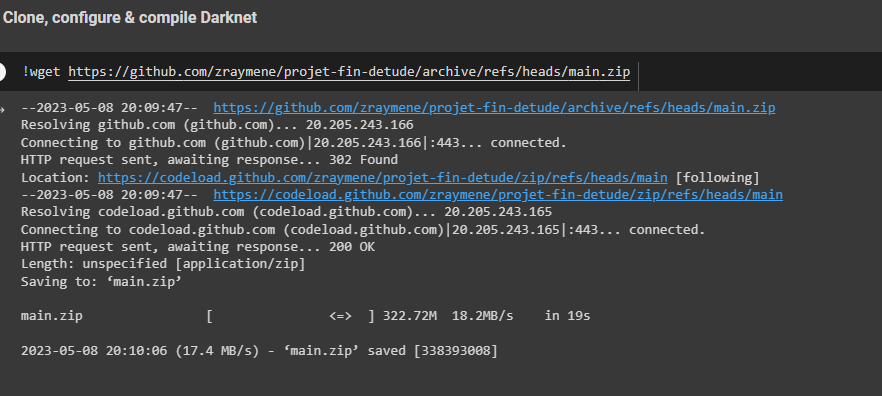
\includegraphics[height=11cm,width=14cm]{Chapitre3/y3-4.png}
               \caption{ Créer le fichier main.zip}
               \label{y3-4}
               \end{figure} 
          
      \paragraph{-} unzip “main.zip” 
      \begin{figure}[H]
           \centering
           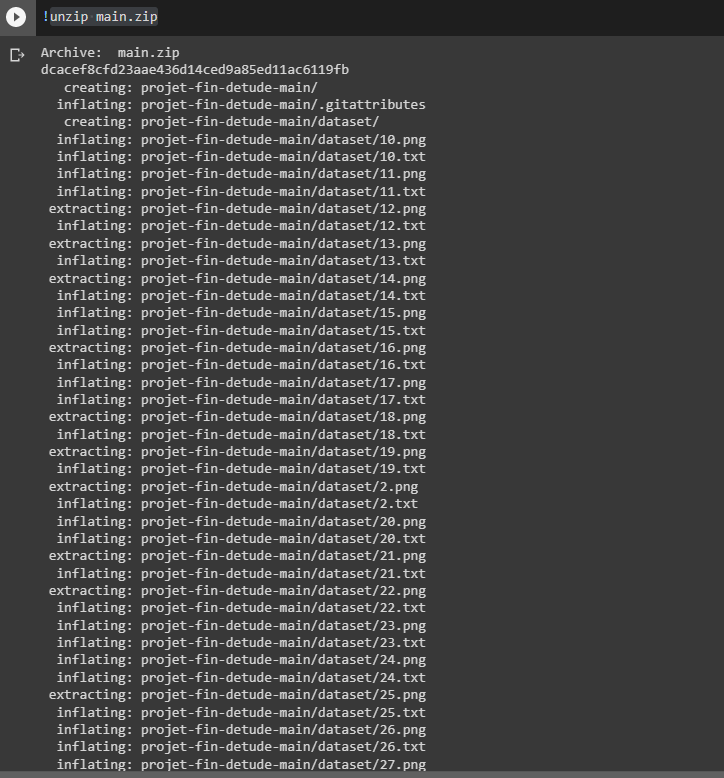
\includegraphics[height=11cm,width=10cm]{Chapitre3/y3-5.png}
           \caption{ unzip le fichier main.zip}
           \label{y3-5}
           \end{figure} 
          
      \paragraph{-}  Copier, configurer et compiler Darknet.
      \begin{figure}[H]
           \centering
           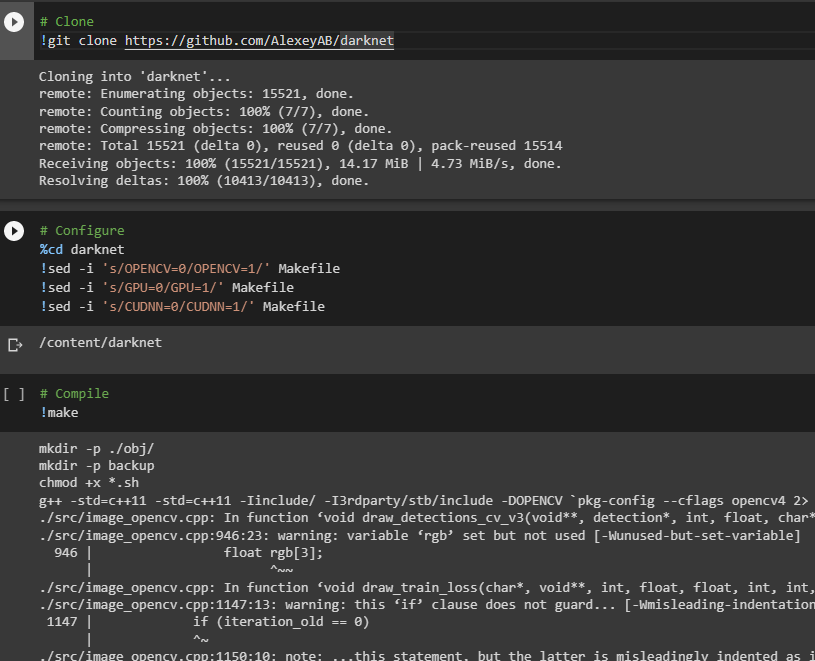
\includegraphics[height=13cm,width=12cm]{Chapitre3/y3-6.png}
           \caption{Darkent}
           \label{y3-6}
           \end{figure}  

      \paragraph{-} Créé  yolov3-training.cfg à partir du fichier yolov3.cfg Toutes les modifications et configurations que nous apporterons à notre modèle personnalisé soient reflétées dans le fichier yolov3-training.cfg
      \begin{figure}[H]
           \centering
           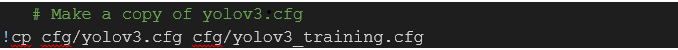
\includegraphics[height=2cm,width=15cm]{Chapitre3/y3-7.png}
           \caption{Créé  yolov3-training.cfg}
           \label{y3-7}
           \end{figure}
      \paragraph{-}  Il y a un seul classe donc [1] : 

      For n = 1: max-batches = 2000, classes=1, filters=18 

      max-batches = 2000 * n and filters = (n + 5) * 3 

      For n = 2: max-batches = 4000, classes=2, filters=21

      For n = 3: max-batches = 8000, classes=3, filters=24
      \begin{figure}[H]
           \centering
           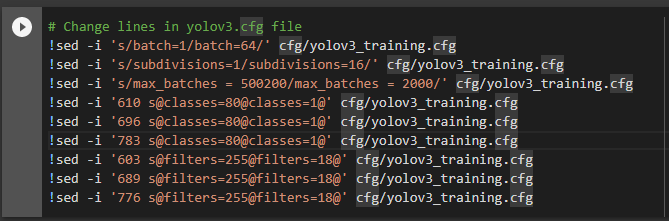
\includegraphics[height=7cm,width=16cm]{Chapitre3/y3-8.png}
           \caption{classes,filters,max-batches }
           \label{y3-8}
           \end{figure} 


      \paragraph{-}  crée les fichiers obj.names et obj.data dans le répertoire darknet/data/obj
      Ces fichiers contiennent des métadonnées telles que les noms des classes et le nombre de classes nécessaires à la formation.       
      \begin{figure}[H]
           \centering
           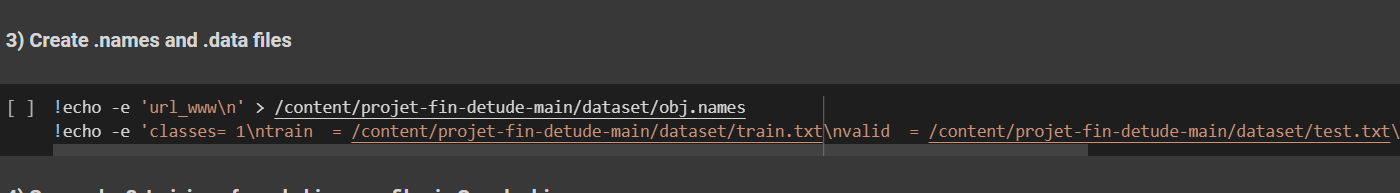
\includegraphics[height=2cm,width=16cm]{Chapitre3/y3-9.png}
           \caption{obj.names et obj.data}
           \label{y3-9}
           \end{figure} 

      \paragraph{-} Enregistrer les fichiers yolov3 training.cfg et  obj.names dans Google Drive et darkent.
      \begin{figure}[H]
           \centering
           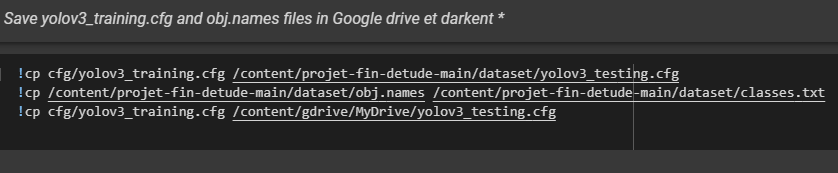
\includegraphics[height=3cm,width=16cm]{Chapitre3/y3-10.png}
           \caption{save yolov3-training.cfg et obj.names }
           \label{y3-10}
           \end{figure} 

      \paragraph{-} création du fichier train.txt  
      Il contient l'emplacement de toutes les images  
      Récupération des images pour traitement
      \begin{figure}[H]
           \centering
           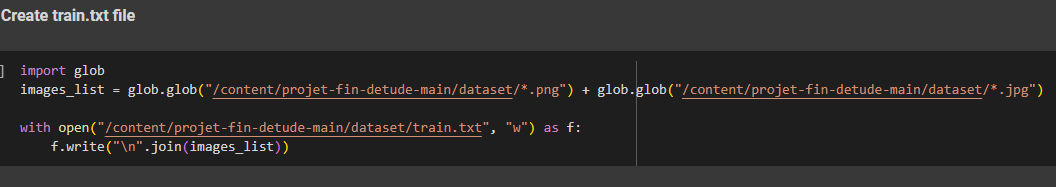
\includegraphics[height=3cm,width=16cm]{Chapitre3/y3-11.png}
           \caption{ fichier train.txt }
           \label{y3-11}
           \end{figure}

      \paragraph{-} Télécharger les poids pré-entraînés pour le fichier des couches convolutives On utilise darknet53.conv.74. : 
      est un  modèle d’apprentissage  déjà formé. C’est utilisé pour forme  à notre modèle.
      Gagner du temps et économiser des calculs dans le processus d'apprentissage.
      \begin{figure}[H]
           \centering
           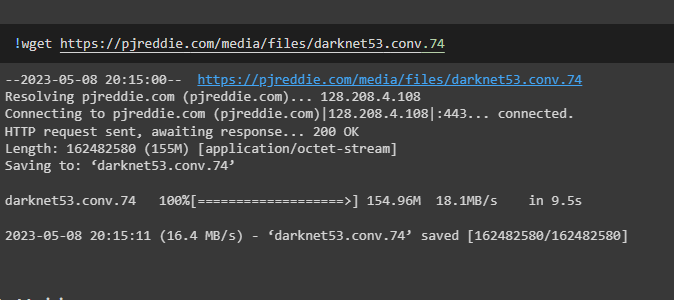
\includegraphics[height=6cm,width=12cm]{Chapitre3/y3-12.png}
           \caption{ Préparer et télécharger  darknet53.conv.74}
           \label{y3-12}
           \end{figure} 

      \paragraph{-} ont commencé le processus d'apprentissage
      L'apprentissage du modèle prendra un certain temps (7 H:43 Min).
      \begin{figure}[H]
            \centering
            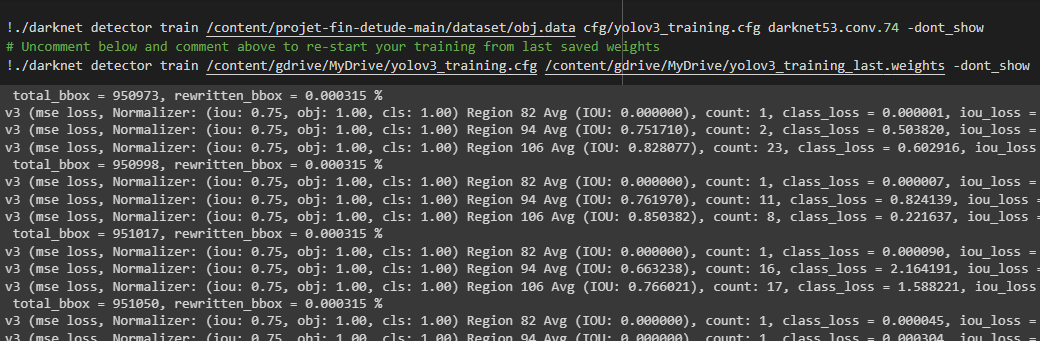
\includegraphics[height=9cm,width=15cm]{Chapitre3/y3-13.png}
            \caption{ le processus d'apprentissage }
            \label{y3-13}
           \end{figure} 
     
      \paragraph{-} À la fin de la formation, il donne 3 fichiers ( yolov3-training - 2000.weights \ yolov3 - training - last.weights /  yolov3 - training - final.weights).
      \begin{figure}[H]
           \centering
           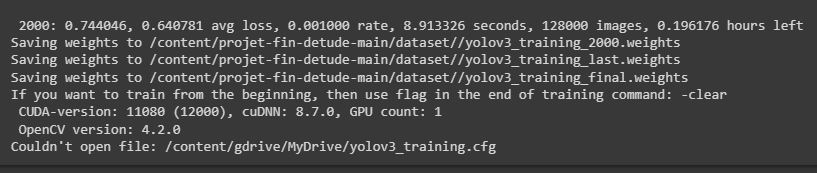
\includegraphics[height=6cm,width=16cm]{Chapitre3/y3-14.png}
           \caption{ le processus d'apprentissage est terminé}
           \label{y3-14}
           \end{figure}

      \paragraph{-} Téléchargez et sauvegardez (yolov3-training-last.weight, classes.txt , yolov3-testing.cfg).
 

     % ------------ YOLOv4 -------------
     \subsection{YOLOv4}
     \paragraph{1-} Nous chargeons d'abord notre jeu de données, cette fois il est chargé depuis Roboflow car il est beaucoup plus facile de le télécharger directement depuis github puis de le décompresser. Roboflow télécharge, décompresse et crée des variables globales python liées à l'ensemble de données, ce qui facilite la configuration de la formation.

     Ce bloc de code est généré automatiquement dans la page roboflow de l'ensemble de données :
     \begin{figure}[H]
               \centering
               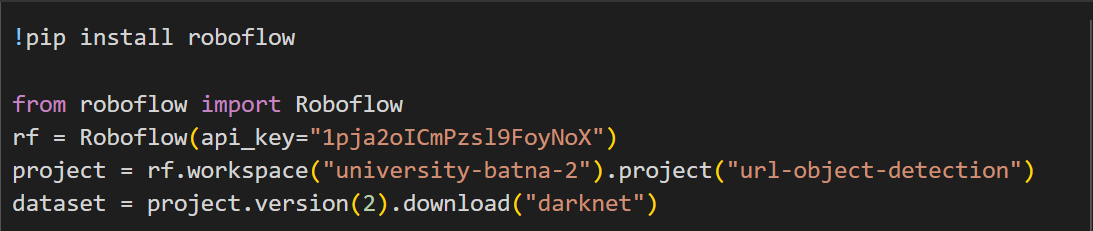
\includegraphics[height=4cm,width=16cm]{Chapitre3/y4_1.png}
               \caption{Commandes pour télécharger l'ensemble de données depuis Roboflow.}
               \label{y4_1}
               \end{figure}
     
     \paragraph{2-} Pour indiquer à Darknet la liste des images de l'ensemble de données, un fichier texte est créé nommé "train.txt" qui contient toutes les images de l'ensemble de données avec leurs fichiers d'annotation. Ce script python automatisera le processus.
     \begin{figure}[H]
               \centering
               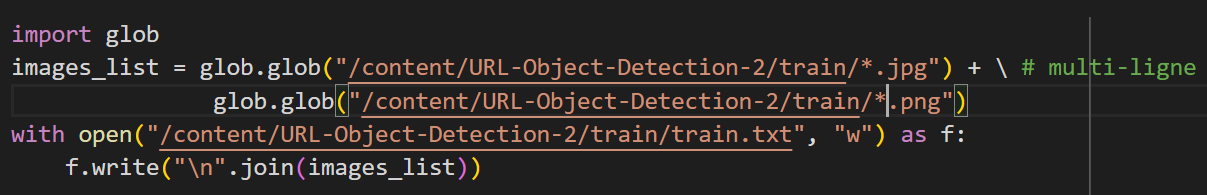
\includegraphics[height=4cm,width=16cm]{Chapitre3/y4_3.png}
               \caption{Script Python pour créer le fichier \(train.txt\).}
               \label{y4_2}
               \end{figure}

     \paragraph{3-} Darknet YOLO enregistre les poids toutes les 500 itérations sur le disque et les machines de collaboration Google ne garantissent pas que l'instance reste ouverte pendant toute la durée de la formation. Pour résoudre ce problème, nous montons notre lecteur Google car il offre un stockage fiable et, dans les étapes ultérieures, nous configurerons le répertoire de sortie pour qu'il soit notre lecteur Google monté.
     \begin{figure}[H]
               \centering
               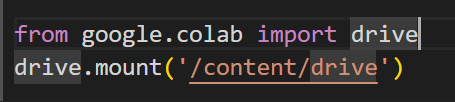
\includegraphics[height=2cm,width=6cm]{Chapitre3/y4_2.png}
               \caption{Script Python pour monter Google Drive sur l'instance actuelle.}
               \label{y4_3}
               \end{figure}

     \paragraph{4-} Maintenant, nous téléchargeons le code source du framework Darknet à partir de github et il est nécessaire de le compiler. Nous nous assurons qu'il est configuré pour utiliser OpenCV et CUDA pour accélérer la formation.
     \begin{figure}[H]
               \centering
               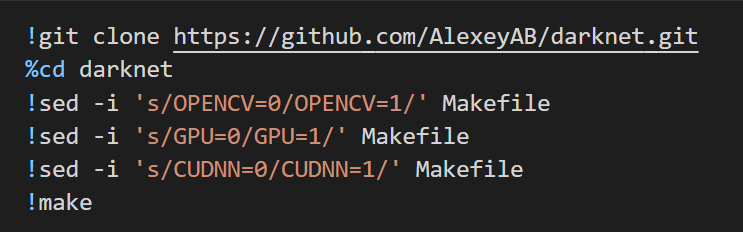
\includegraphics[height=6cm,width=14cm]{Chapitre3/y4_4.png}
               \caption{Télécharger et compiler Darknet.}
               \label{y4_4}
               \end{figure}

     \paragraph{5-} Pour configurer le framework Darknet, 2 fichiers doivent être créés. Le premier est \(obj.data\) qui contient :
     \paragraph{-} Nombre de cours

     \paragraph{-} Fichier contenant la liste des images du jeu de données et leur fichier d'annotation pour la formation et les tests, qui est \(train.txt\) que nous avons créé auparavant. (nous utiliserons notre formation personnalisée afin qu'il ne soit pas nécessaire de définir l'attribut de test)
     \paragraph{-} Fichier contenant les noms des classes (sera créé prochainement) .
     \paragraph{-} Répertoire où seront sauvegardés les poids (ce sera le google drive monté).
     
     Le deuxième fichier est \(obj.names\) où les noms des classes seront définis, chaque ligne définit une classe.
     Les deux fichiers seront placés dans le répertoire \(cfg/\).
     \begin{figure}[H]
               \centering
               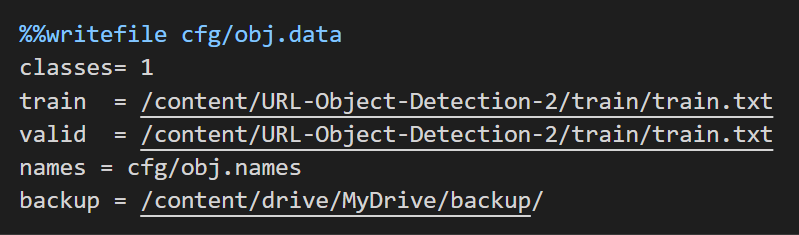
\includegraphics[height=6cm,width=14cm]{Chapitre3/y4_5.png}
               \caption{Creation de fichier \(obj.data\).}
               \label{y4_5}
               \end{figure}
               
      \begin{figure}[H]
               \centering
               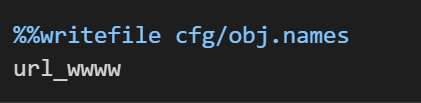
\includegraphics[height=2cm,width=6cm]{Chapitre3/y4_5_5.png}
               \caption{Creation de fichier \(obj.names\).}
               \label{y4_5_5}
               \end{figure}
           
     
     \paragraph{6-} Pour configurer notre réseau, nous allons modifier le fichier de configuration \(yolov4-custom.cfg\) qui se trouve dans le répertoire \(cfg/\). Les configurations qui nous concernent sont :
     \paragraph{-} \(batch\): définit le nombre d'images traitées en 1 itération (mise à jour du poids), contrairement aux ecpoches où l'ensemble des données est entièrement itéré.
     \paragraph{-} \(sous-divisions\): la mémoire GPU n'est pas infinie, il est donc impossible de passer un lot complet à la mémoire GPU pour le traitement. Subdiviser le lot en mini-lot est la solution. les sous-divisions inférieures sont les besoins en mémoire GPU les plus élevés, si la mémoire n'est pas suffisante, une erreur sera renvoyée au début de la formation.
     \paragraph{-} \(max-batches\): cette valeur définit le nombre d'itérations lorsque la formation s'arrêtera. \(2000 * number_classes\) est recommandé pour de meilleurs résultats.
     \paragraph{-} \(classes\) : définit le nombre de classes que le réseau formera. trouvé dans les lignes: $970$, $1058$ et $1146$.
     \paragraph{-} \(filtres\) : cela définit la taille des filtres trouvés avant un $[yolo]$ sur la configuration. trouvé dans les lignes : $963$, $1051$ et $1139$. La taille du filtre suit la formule suivante : $(nombre-classes + 5) * 3$
     \begin{figure}[H]
               \centering
               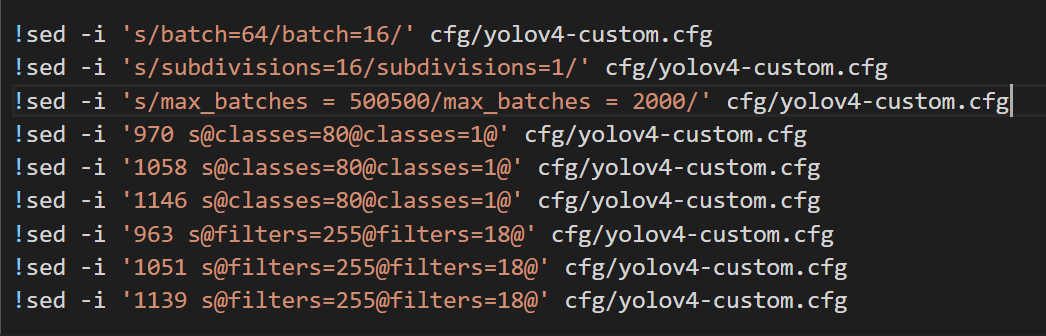
\includegraphics[height=8cm,width=16cm]{Chapitre3/y4_6.png}
               \caption{Script pour modifier le fichier de configuration $cfg/yolov4-custom.cfg$.}
               \label{y4_6}
               \end{figure}
     
     \paragraph{7-} Après avoir configuré le réseau, les poids pré-formés sont téléchargés pour appliquer l'apprentissage par transformation.
     \begin{figure}[H]
               \centering
               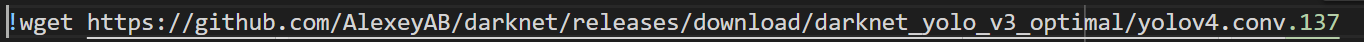
\includegraphics[height=0.5cm,width=17cm]{Chapitre3/y4_7.png}
               \caption{Téléchargés les poids pré-formés.}
               \label{y4_7}
               \end{figure}
      
     \paragraph{8-} Enfin, nous lançons notre formation avec la commande suivante. il faudra des heures pour terminer.
     \begin{figure}[H]
               \centering
               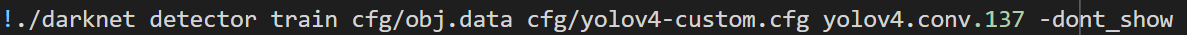
\includegraphics[height=0.5cm,width=17cm]{Chapitre3/y4_8.png}
               \caption{Commencez l'entraînement en sélectionnant les poids pré-entraînés.}
               \label{y4_8}
               \end{figure}
      
     \paragraph{Condition spéciale :} si l'entraînement échoue à mi-parcours en raison de la désactivation de l'instance Google Colab. l'entraînement peut être poursuivi en utilisant les derniers poids enregistrés qui ont été enregistrés sur Google Drive en modifiant la commande de train pour utiliser le dernier poids.
     \begin{figure}[H]
               \centering
               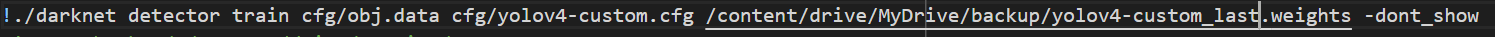
\includegraphics[height=0.5cm,width=17cm]{Chapitre3/y4_9.png}
               \caption{Continue la formation.}
               \label{y4_9}
               \end{figure}
      
               

     % ------------ YOLOv5 -------------
     \subsection{YOLOv5}
     \paragraph{1-} YOLOv5 améliore l'accessibilité et la facilité d'utilisation, cette commande suivante téléchargera le code source YOLOv5 à partir de Github et téléchargera les bibliothèques Python requises, y compris PyTorch.
     \begin{figure}[H]
               \centering
               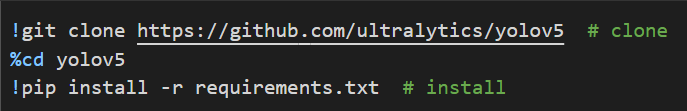
\includegraphics[height=2cm,width=12cm]{Chapitre3/y5_1.png}
               \caption{Commandes pour télécharger YOLOv5 et installer Python requis}
               \label{y5_1}
               \end{figure}
               
     \paragraph{2-} Maintenant que nous téléchargeons notre ensemble de données, Roboflow se chargera de convertir notre format d'ensemble de données dans le format que YOLOv5 peut utiliser.
     \begin{figure}[H]
               \centering
               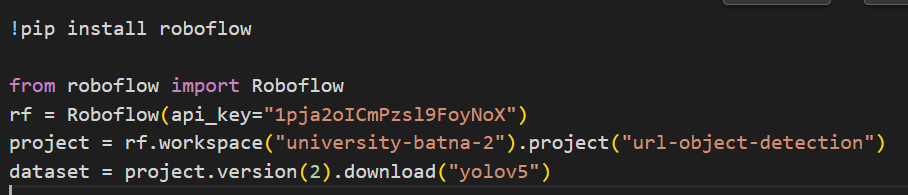
\includegraphics[height=4cm,width=16cm]{Chapitre3/y5_2.png}
               \caption{Commandes pour télécharger l'ensemble de données depuis Roboflow.}
               \label{y5_2}
               \end{figure}
               
     \paragraph{3-} Enfin nous commençons la formation, nous pouvons paramétrer configurer notre formation en passant des arguments à la commande comme :
     \paragraph{-} $img-size$ : les dimensions de l'image d'entrée.
     \paragraph{-} $epochs$ : nombre d'itérations complètes du jeu de données. Contrairement à YOLOv3 et YOLOv4, YOLOv5 itère sur l'ensemble de données en 1 époque.
     \paragraph{-} $batch$ : nombre d'images dans un lot. YOLOv5 divise l'ensemble de données en lots en raison des limitations de la mémoire GPU
     \paragraph{-} $weights$ : poids pré-entraînés du modèle YOLOv5. YOLOv5 a plusieurs modèles allant des modèles nano avec une petite taille et une vitesse dans le coût de précision au modèle XLarge avec une plus grande précision mais une plus grande taille.
     \begin{figure}[H]
               \centering
               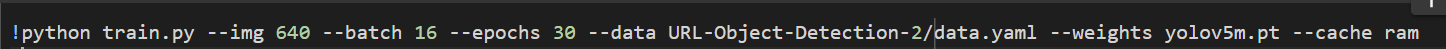
\includegraphics[height=0.5cm,width=17cm]{Chapitre3/y5_3.png}
               \caption{Lancer l'entraînement de YOLOv5.}
               \label{y5_3}
               \end{figure}

     \subsection{Outil Utiliser}
               \subsubsection{Google Collab:} est un outil d'analyse de données et d'apprentissage automatique qui vous permet de combiner du code Python exécutable et du texte enrichi avec des 	graphiques, des images, HTML, LaTeX et plus encore dans un seul document stocké dans Google Drive. Il se connecte aux puissants environnements d'exécution de Google Cloud Platform et vous permet de partager facilement votre travail et de collaborer avec d'autres.
               \subsubsection{Python:} est un langage de programmation généraliste de haut niveau. Sa philosophie de conception met l'accent sur la lisibilité du code avec l'utilisation d'une indentation significative via la règle du hors-jeu. Python est dynamiquement typé et ramassé. Il est utilisé pour créer des scripts pour automatiser les processus. 
               \subsubsection{Darknet:} est un framework de réseau neuronal open source écrit en C et CUDA et prend en charge le calcul CPU et GPU. il était utilisé pour entraîner les modèles de détection d'objets YOLOv3 et YOLOv4.
               \subsubsection{PyTorch:} est open-source gratuit et un cadre d'apprentissage automatique basé sur la bibliothèque Torch, utilisé pour des applications telles que la vision par ordinateur et le traitement du langage naturel.


% ========= TESING =============
\section{Testing}
     Tous les modèles sont formés sur le même jeu de données qui contient 127 images et tous seront évalués sur des images de test.
     Nous voulons tester comment les modèles réagissent à différents types de :
     \paragraph{-} Police de caractère.
     \paragraph{-} Couleur.
     \paragraph{-} Transformation (Rotation).
     \paragraph{-} URL avec préfixe de protocole https
     \paragraph{-} Manuscrits.
     
     La métrique d'évaluation finale est la précision moyenne (AP) qui donne des performances précises du modèle qui est calculé à partir de la courbe de rappel de précision
     Le seuil d'intersection sur union (IoU) est $0.5$.

     % ---------- YOLOv3 -------------
     \subsection{YOLOv3}
     En général,, le modèle a donné $43.12\%$ comme précision moyenne (AP). 
      \begin{figure}[H]
               \centering
                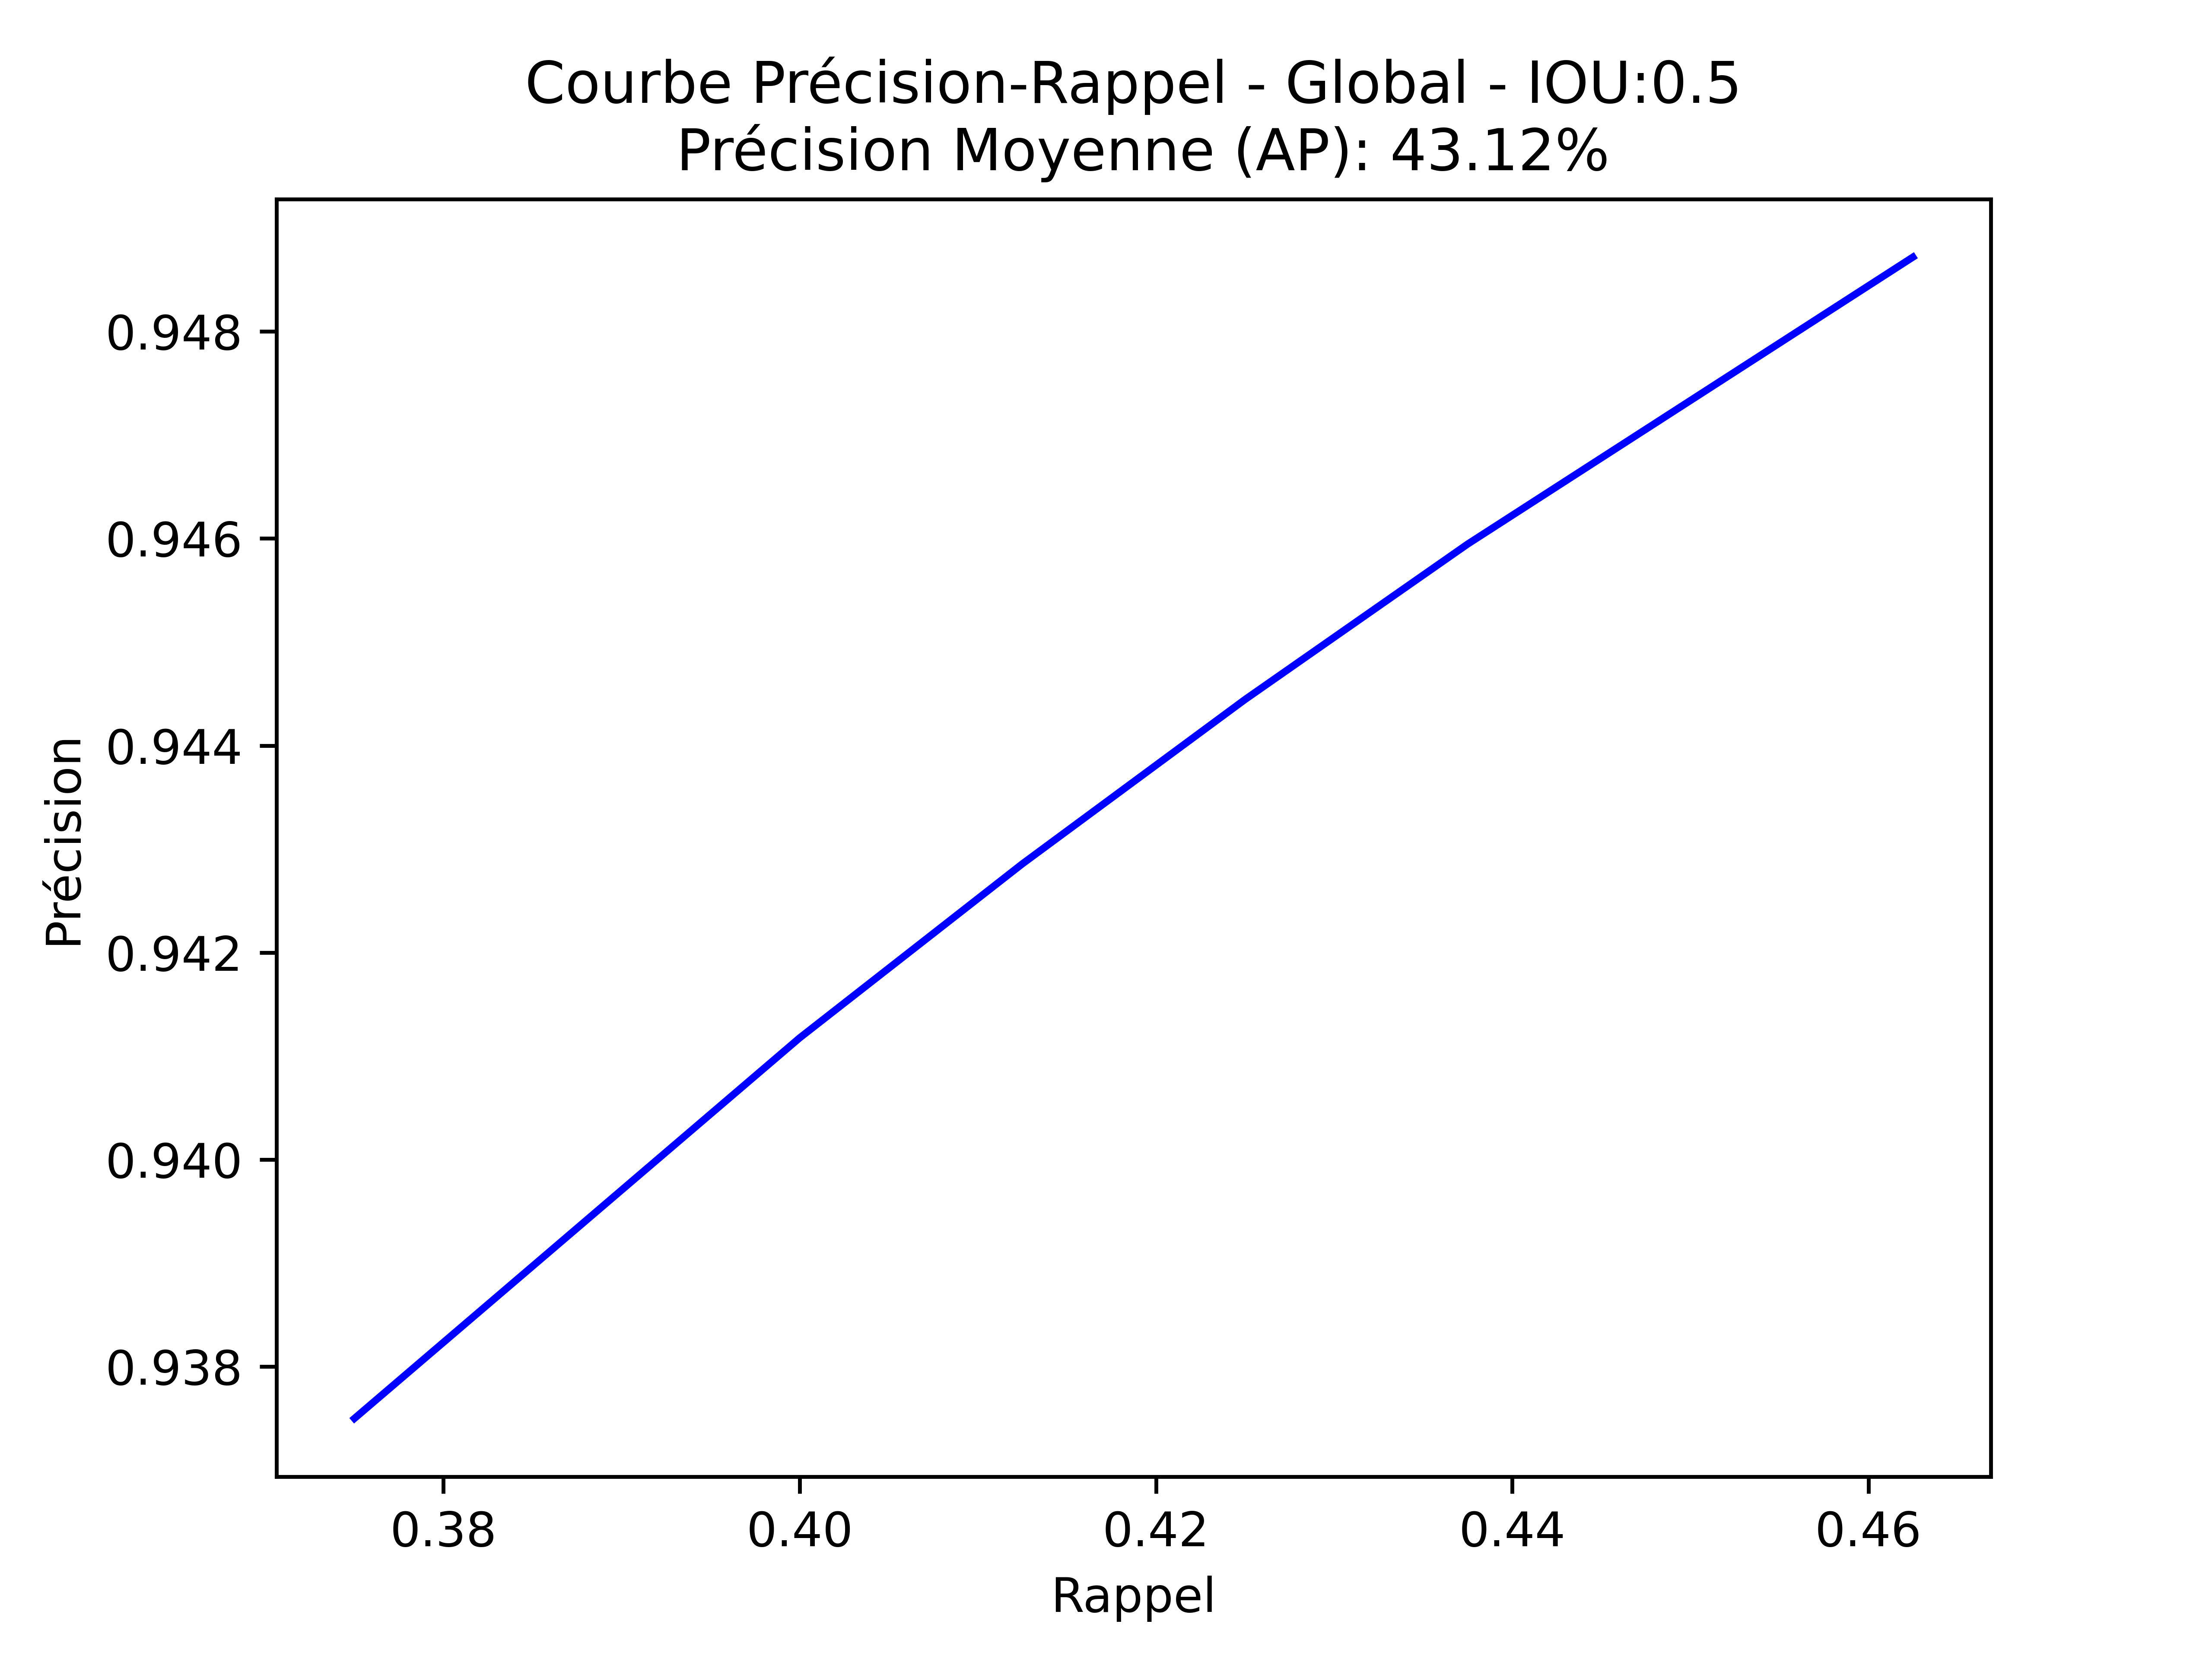
\includegraphics[height=10cm,width=17cm]{Chapitre3/yolov3-pr-Global.png}
                \caption{YOLOv3: Courbe Précision-Rappel et Précision Moyenne de modele.}
                \label{y3_t0}
                \end{figure}

      \paragraph{1-} Police de caractère.
         Il y  3 types des polices  et nous allons faites des tests par yolo-v3 et afficher les résultats.
      \begin{figure}[H]
              \centering
               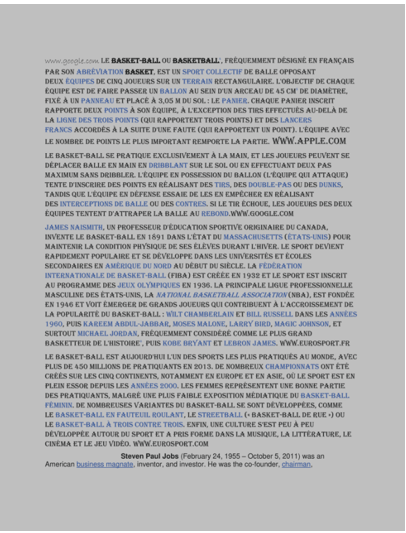
\includegraphics[height=8cm,width=14cm]{Chapitre3/y3-t2.png}
               \caption{YOLOv3: Test des URL écrites en police Arial.}
               \label{y3_t1}
               \end{figure}
       
      \paragraph{-}Le résultat 
      la précision moyenne de l'algorithme yolo-v3 dans cette partie est $72.73\%$.

      \paragraph{2-} Couleur.
      \paragraph{-}  On utilise 15 éléments ont couleurs
       Le résultat qui nous avons détecté et trouver est 7 éléments,  la précision moyenne est de $31.17\%$
      \begin{figure}[H]
          \centering
           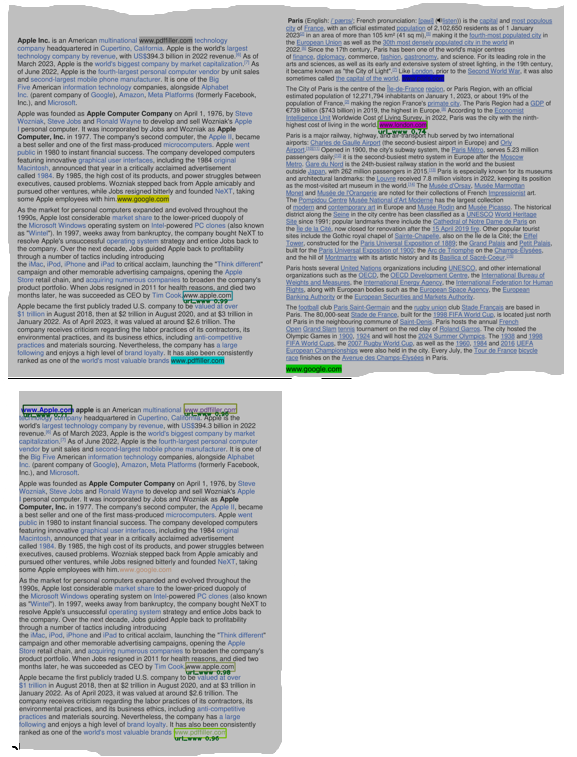
\includegraphics[height=10cm,width=14cm]{Chapitre3/y3-t3.png}
           \caption{YOLOv3: test des URL écrites dans différentes couleurs.}
           \label{y3_t3}
           \end{figure}
     
      \paragraph{3-} Transformation (Rotation).
      \paragraph{-} Pour la rotation de 90 ne donne aucun résultat.
      \begin{figure}[H]
          \centering
           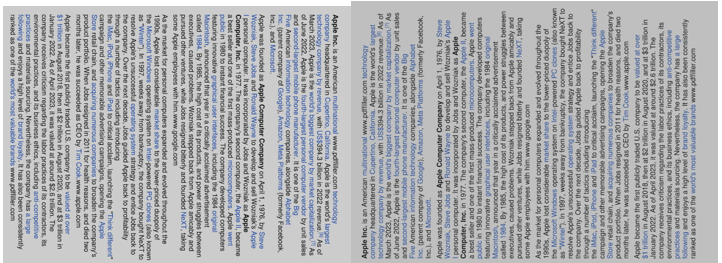
\includegraphics[height=10cm,width=12cm]{Chapitre3/y3-t5.png}
           \caption{YOLOv3: test des URL écrites en rotation $90°$.}
           \label{y3_t5}
           \end{figure}
     
      \paragraph{-} Pour une rotation de 180, le score est $27.27\%$.
      \begin{figure}[H]
          \centering
           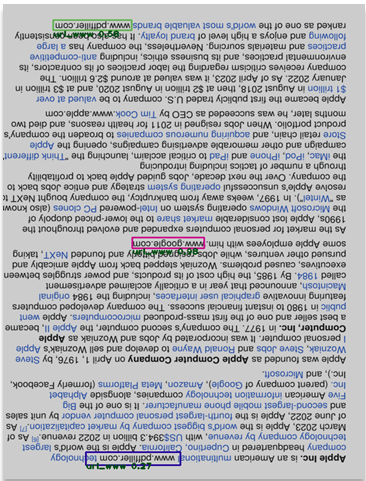
\includegraphics[height=10cm,width=12cm]{Chapitre3/y3-t6.png}
           \caption{YOLOv3: test des URL écrites en rotation $180°$.}
           \label{y3_t6}
           \end{figure}

      \paragraph{3-}Link (https)
      \paragraph{-} Dans cette étude, nous constatons que  la précision moyenne  est faible $12.12\%$ et nous avons remarqué que dans certains cas, nous avons détecté le modèle $www$ dans le modèle $http$.
      
      \begin{figure}[H]
          \centering
           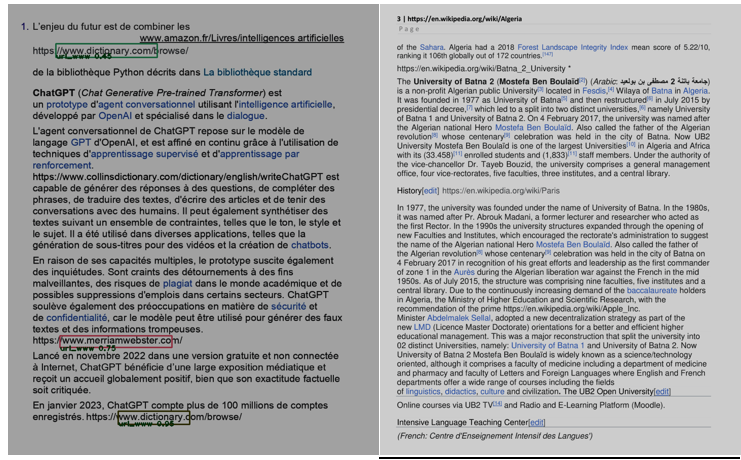
\includegraphics[height=10cm,width=12cm]{Chapitre3/y3-t4.png}
           \caption{yolov3 : tester les URL écrites avec prefixe protocol HTTPS.}
           \label{y3_t4}
           \end{figure}


      \paragraph{4-} Manuscrits.
      \paragraph{-} Dans cette étude, nous n'avons pas obtenu de résultats.

      \begin{figure}[H]
          \centering
           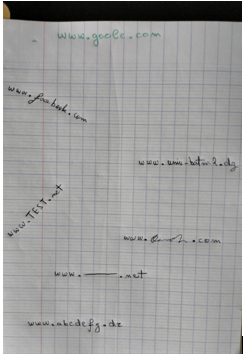
\includegraphics[height=10cm,width=12cm]{Chapitre3/y3-t7.png}
           \caption{YOLOv3: Test des URL écrites en manuscrit.}
           \label{y3_t7}
           \end{figure}

      \paragraph{Conclusion:} Ces résultats nous permettent de dire que Yolov3 a été capable d'obtenir d'excellents résultats malgré les changements dans les images.     

     % ---------- YOLOv4 -------------
     \subsection{YOLOv4}
     Ce modèle est formé en utilisant 16 images par lot et 2000 lots maximum.

     Généralement, le modèle a atteint $53,12\%$ en tant que précision moyenne (AP)
     \begin{figure}[H]
               \centering
               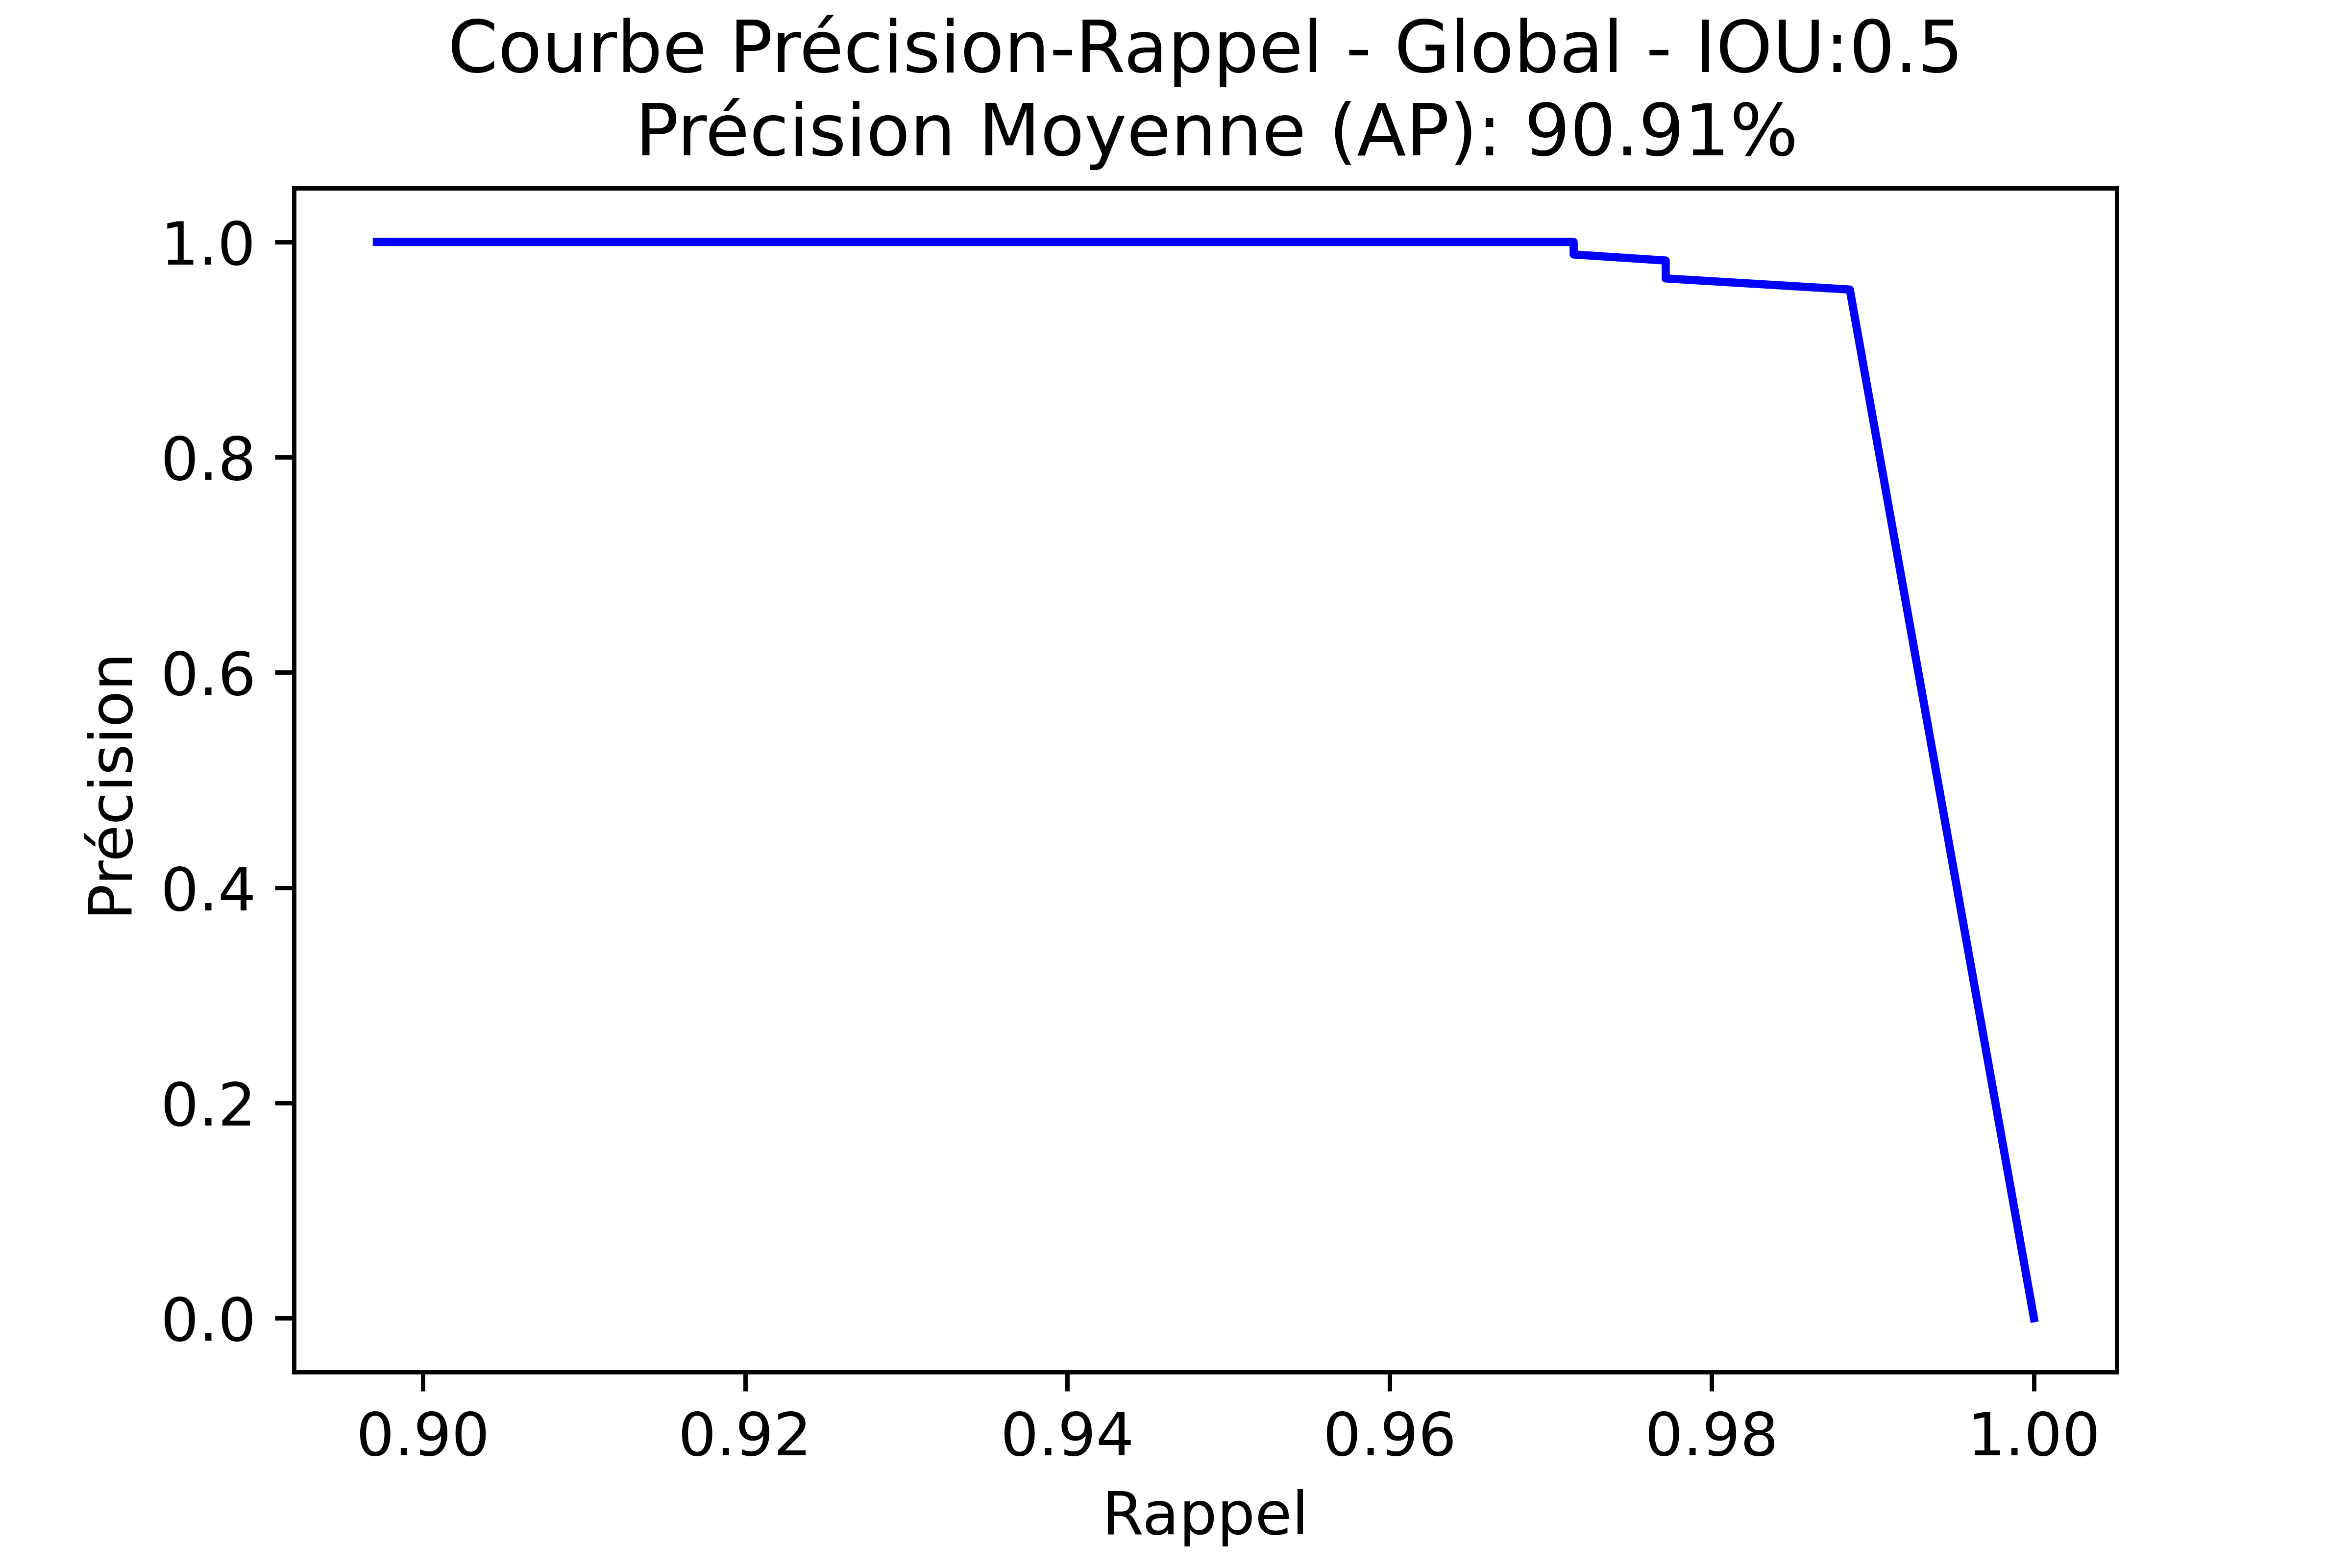
\includegraphics[height=10cm,width=17cm]{Chapitre3/yolov4_pr_global.png}
               \caption{YOLOv4: Courbe Précision-Rappel et Précision Moyenne de modele.}
               \label{y4_pr}
               \end{figure}
     
     Le modèle atteint une précision de moyenne $100.00\%$ sur les ULR écrits en police Arial. L'épaisseur des lettres n'affecte pas les résultats. Cependant, plus l'image est réduite à une taille plus petite, plus la précision diminue.
     \begin{figure}[H]
               \centering
               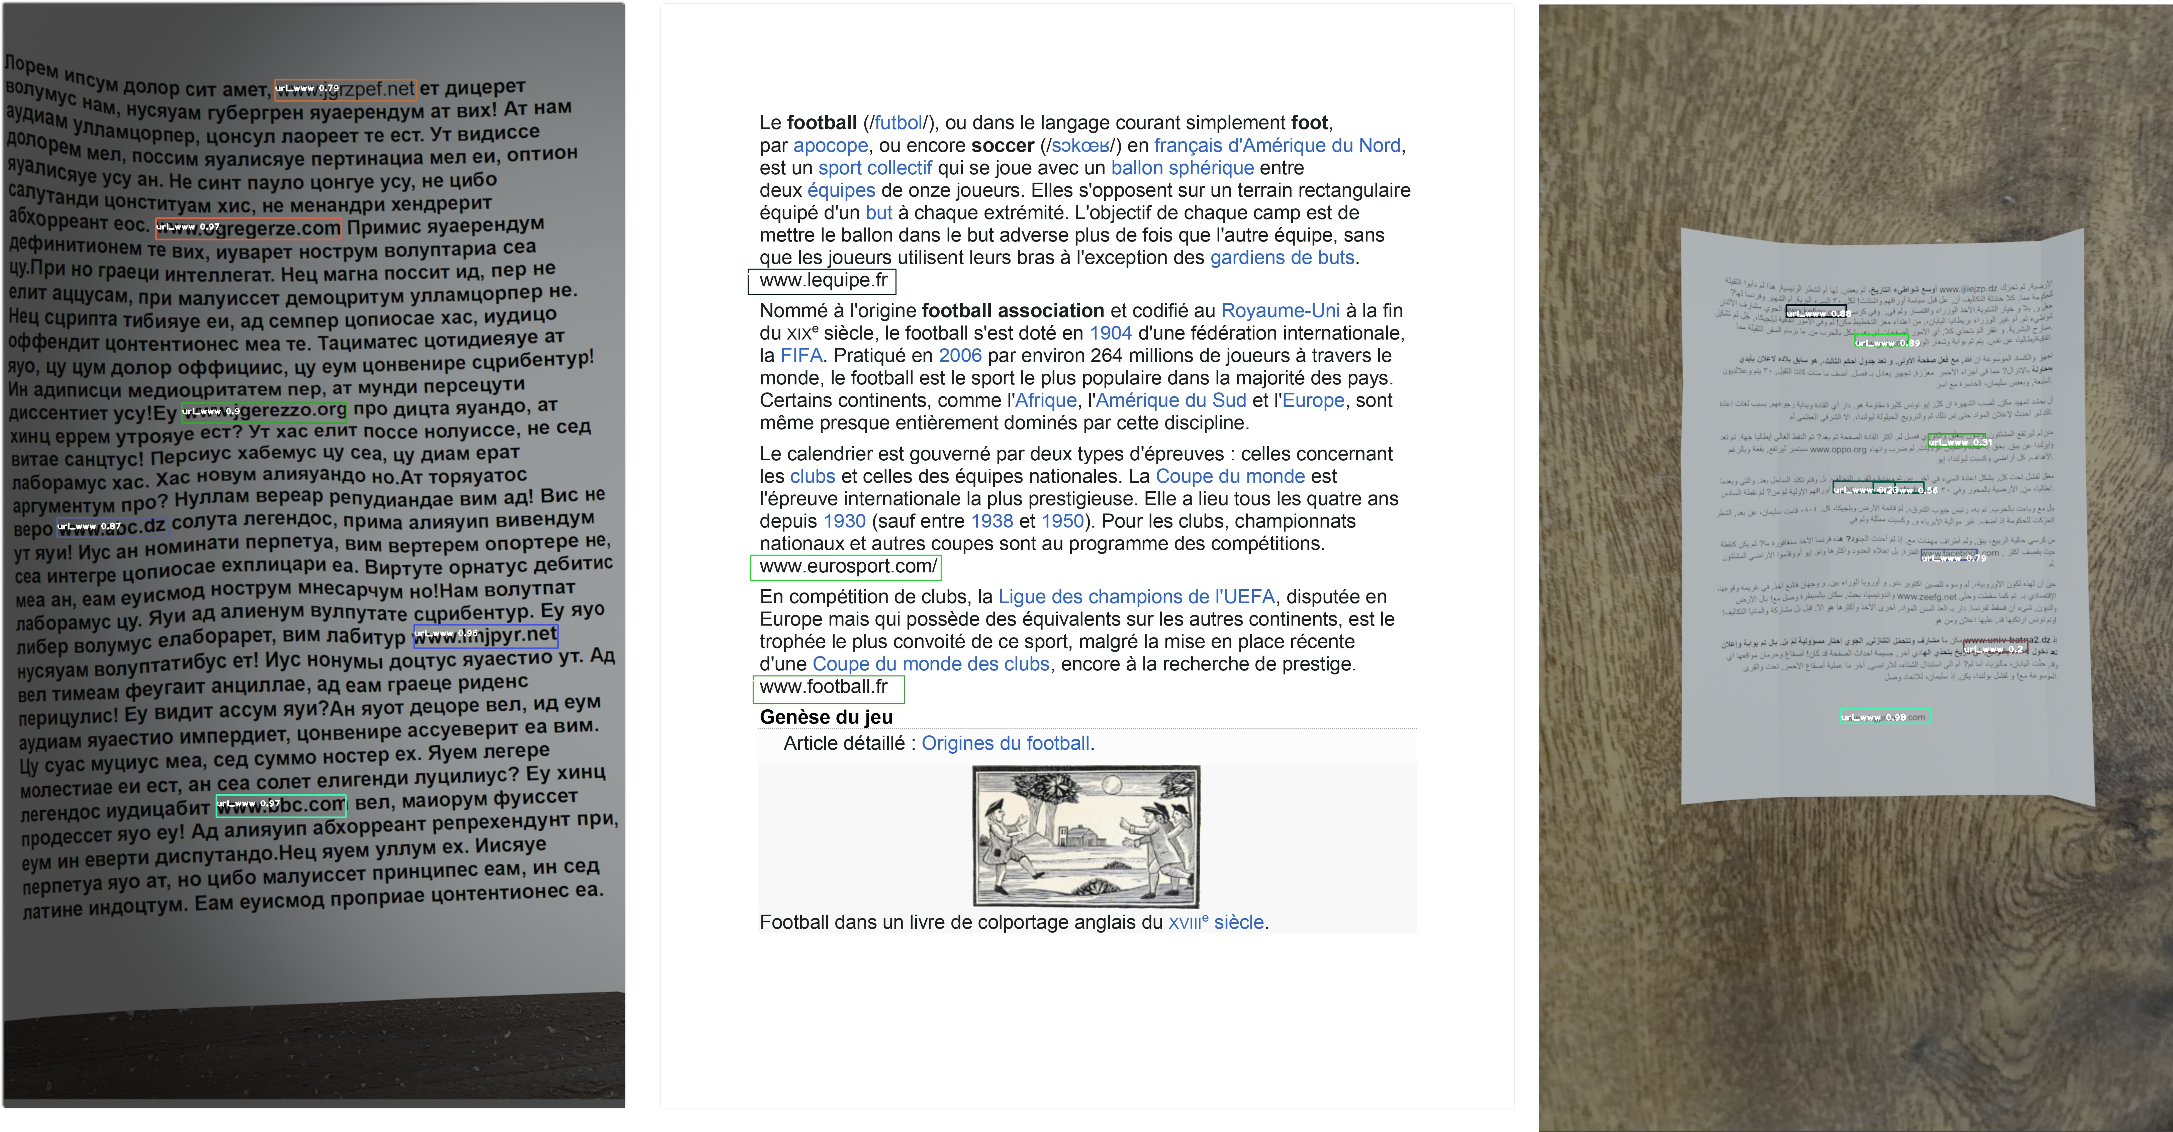
\includegraphics[height=8cm,width=17cm]{Chapitre3/y4_t1.png}
               \caption{YOLOv4 : Test des URL écrites en police Arial.}
               \label{y4_t1}
               \end{figure}
     
     Le modèle atteint une précision moyenne de $84.29\%$ sur les URL écrites dans différentes polices.
     \begin{figure}[H]
               \centering
               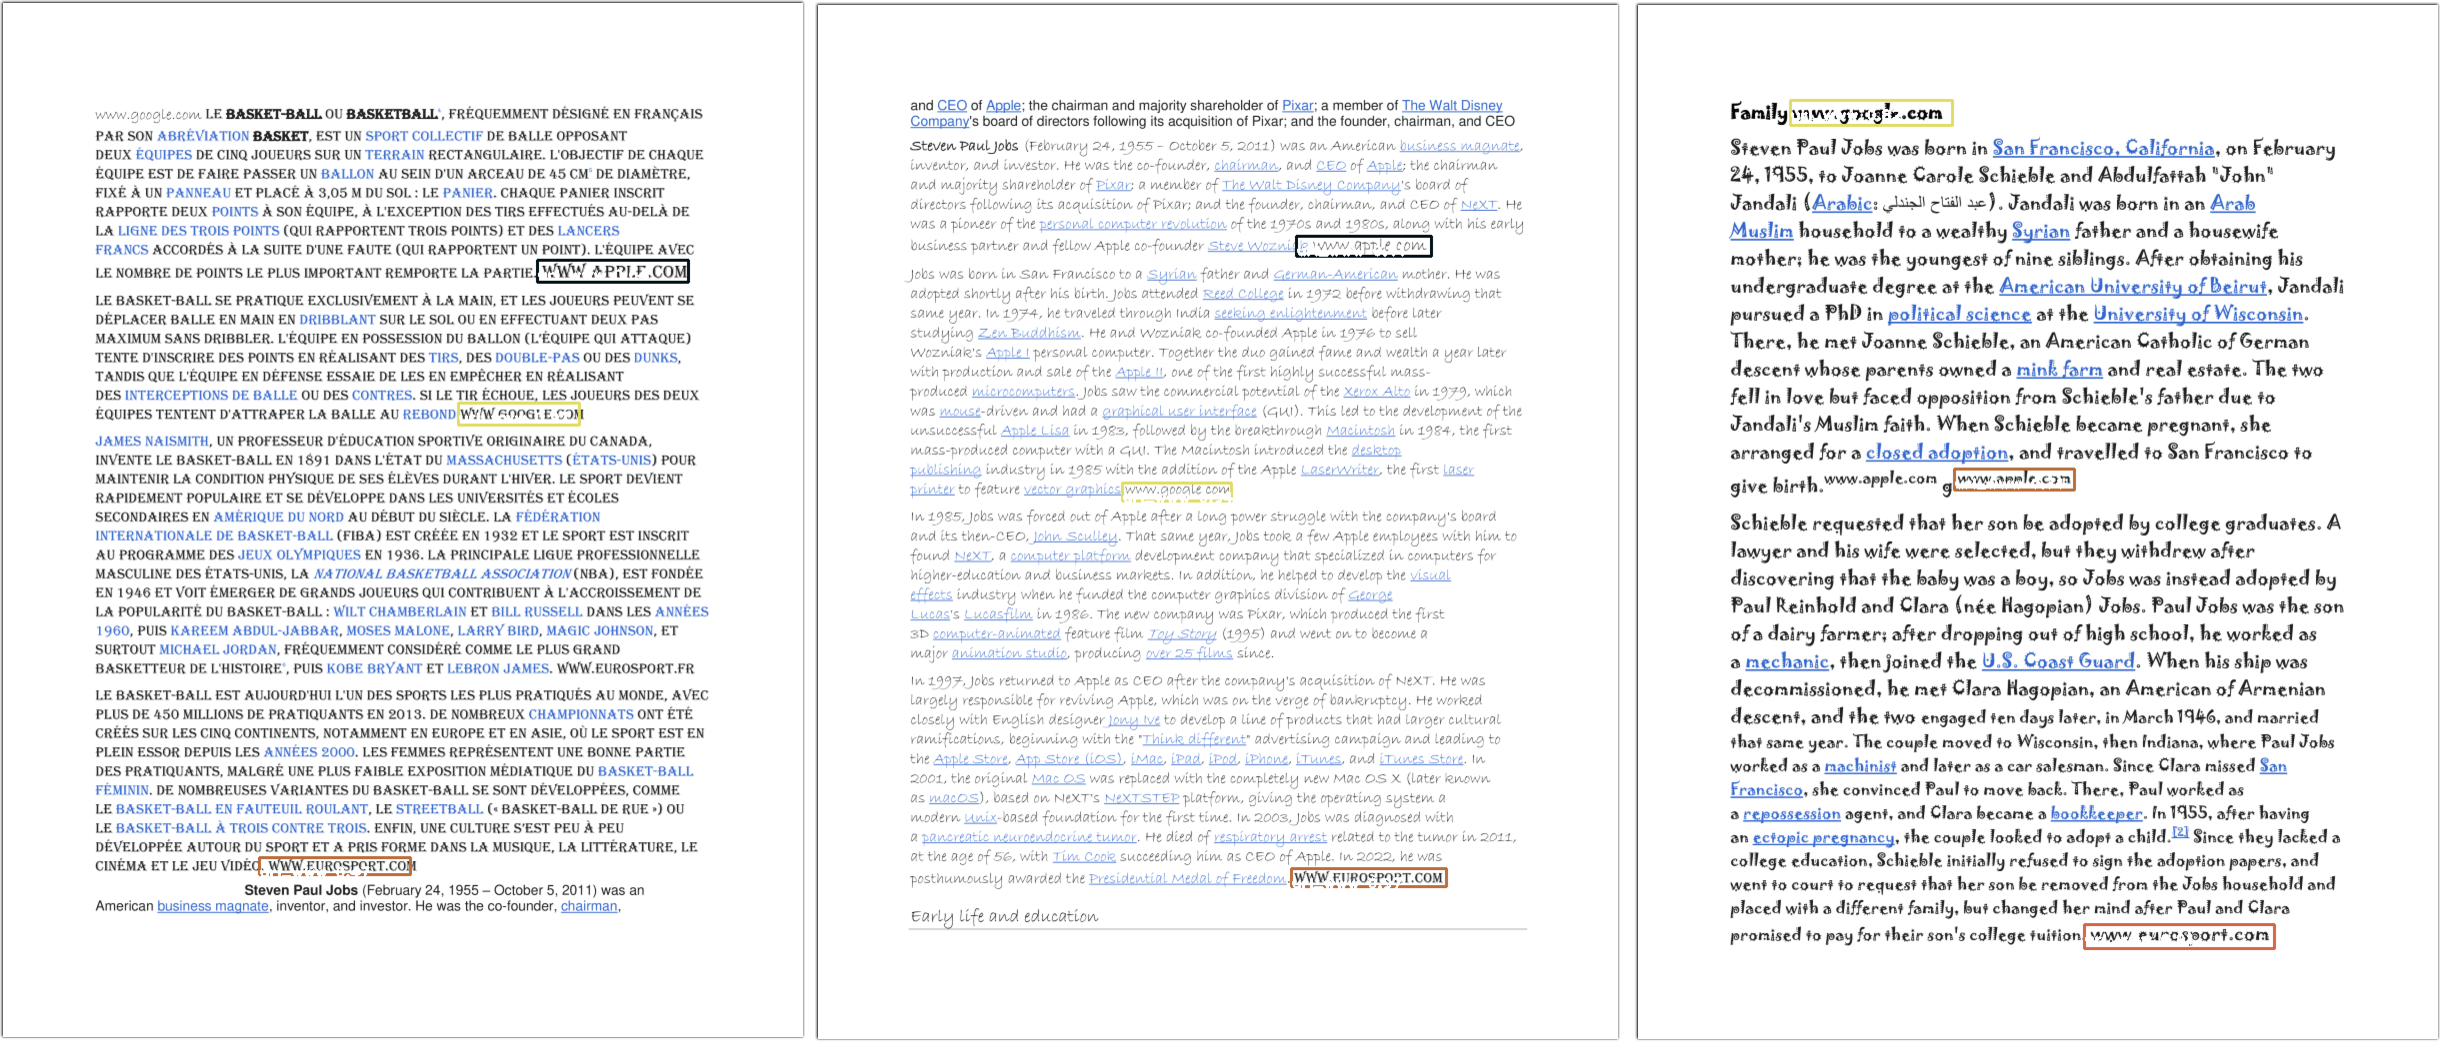
\includegraphics[height=8cm,width=17cm]{Chapitre3/y4_t2.png}
               \caption{YOLOv4 : Test des URL écrites dans différentes polices.}
               \label{y4_t2}
               \end{figure}

     Le modèle atteint une précision moyenne de $54.44\%$ avec des URL de couleurs différentes (lettres et arrière-plan).
     \begin{figure}[H]
               \centering
               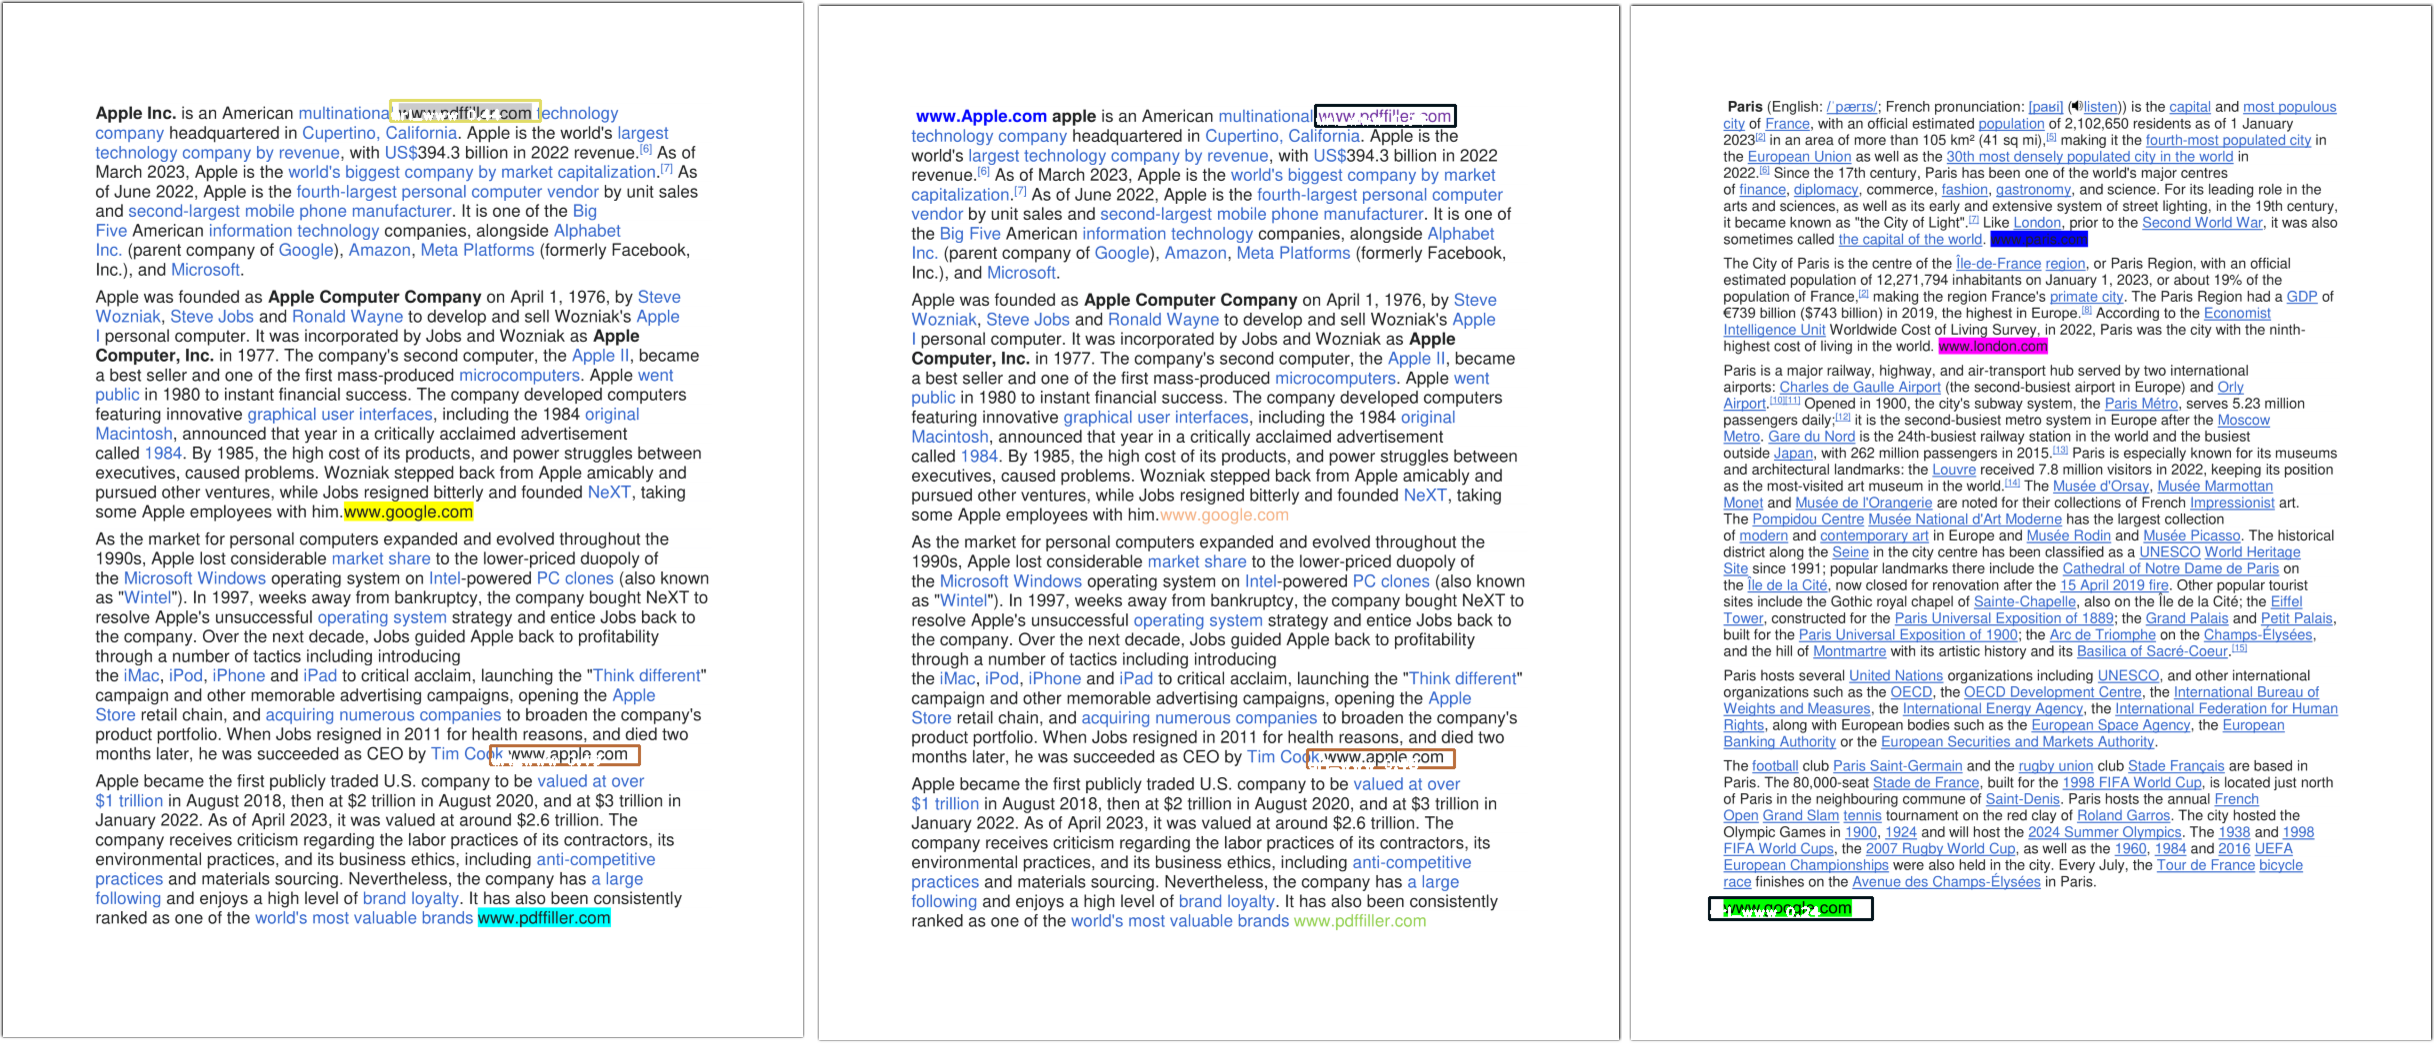
\includegraphics[height=9cm,width=17cm]{Chapitre3/y4_t3.png}
               \caption{YOLOv4 : test des URL écrites dans différentes couleurs.}
               \label{y4_t3}
               \end{figure}

     Dans le cas des rotations, les modèles échouent totalement lorsque l'entrée est tournée de $90°$, d'autre part, une rotation de $180°$ n'affecte pas la précision du modèle.
     \begin{figure}[H]
               \centering
               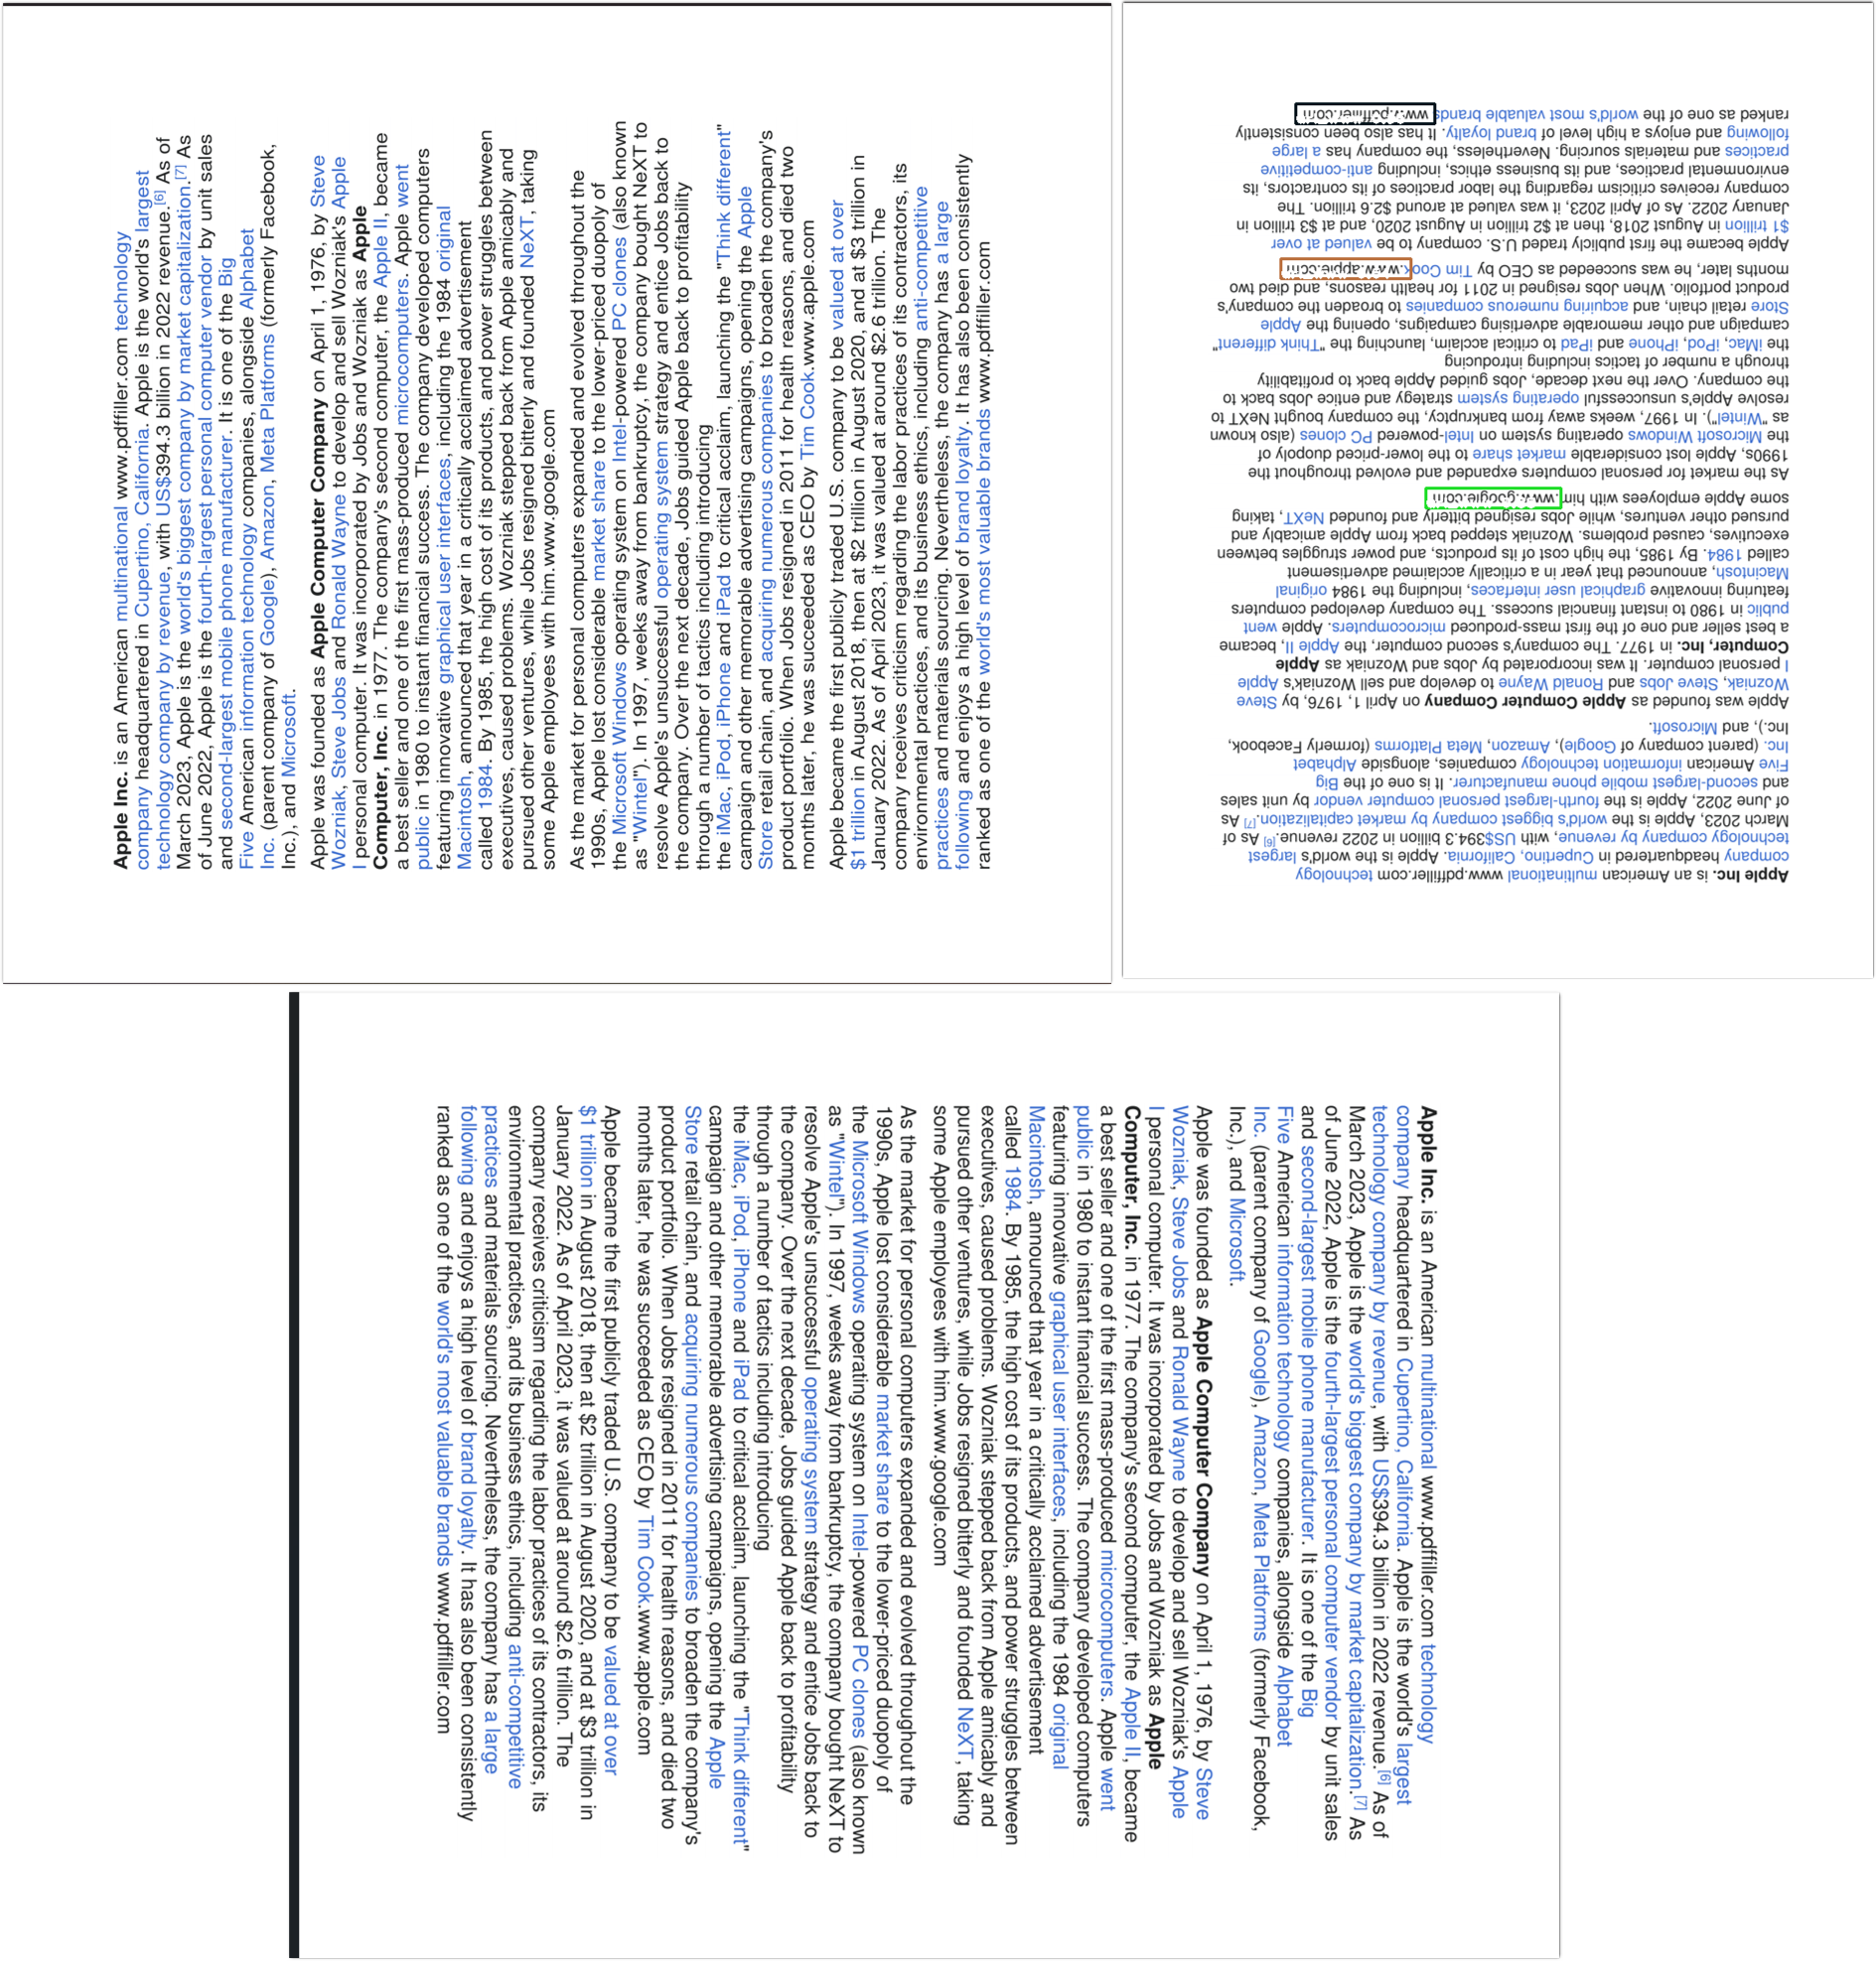
\includegraphics[height=12cm,width=16cm]{Chapitre3/y4_t4.png}
               \caption{YOLOv4 : test des URL écrites dans différentes rotations.}
               \label{y4_t4}
               \end{figure}
     
     Dans le cas d'URL avec le protocole de préfixe https, le modèle ne parvient pas à donner des prédictions précises avec $28.9\%$ précision moyenne
     \begin{figure}[H]
               \centering
               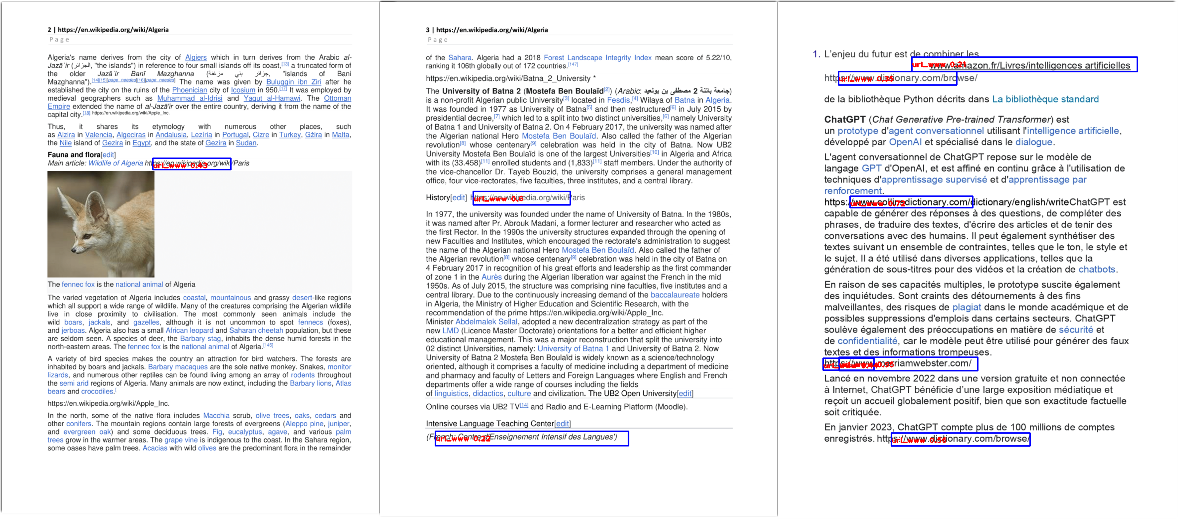
\includegraphics[height=9cm,width=17cm]{Chapitre3/yolov4_https.png}
               \caption{YOLOv4 : test des URL écrites avec prefixe protocol HTTPS.}
               \label{y4_https}
               \end{figure}
     
     Enfin, le modèle ne parvient pas à détecter les URL écrites en manuscrit.
     \paragraph{Conclusion:} Le modèle est fortement affecté par la mise à l'échelle, plus la taille est petite, plus la précision du modèle est faible. Différentes polices réduisent la précision du modèle, mais en plus petites quantités $~ 5\%$. Les couleurs affectent fortement la précision des modèles à la fois en cas de lettres colorées et de couleur de fond. Pour la rotation, les rotations à $90 degrés$ cassent le modèle à $180 degrés$, la précision n'est pas affectée. Enfin, les URL des manuscrits ne sont pas reconnaissables par le modèle, même les faux objets de vérité n'ont pas été détectés.
     
     % ---------- YOLOv5 -------------
     \subsection{YOLOv5}
     Ce modèle a été formé avec 640x640 comme image d'entrée et 30 époques.
     
     Généralement, le modèle a atteint $44,19\%$ en tant que précision moyenne (AP)
     \begin{figure}[H]
               \centering
               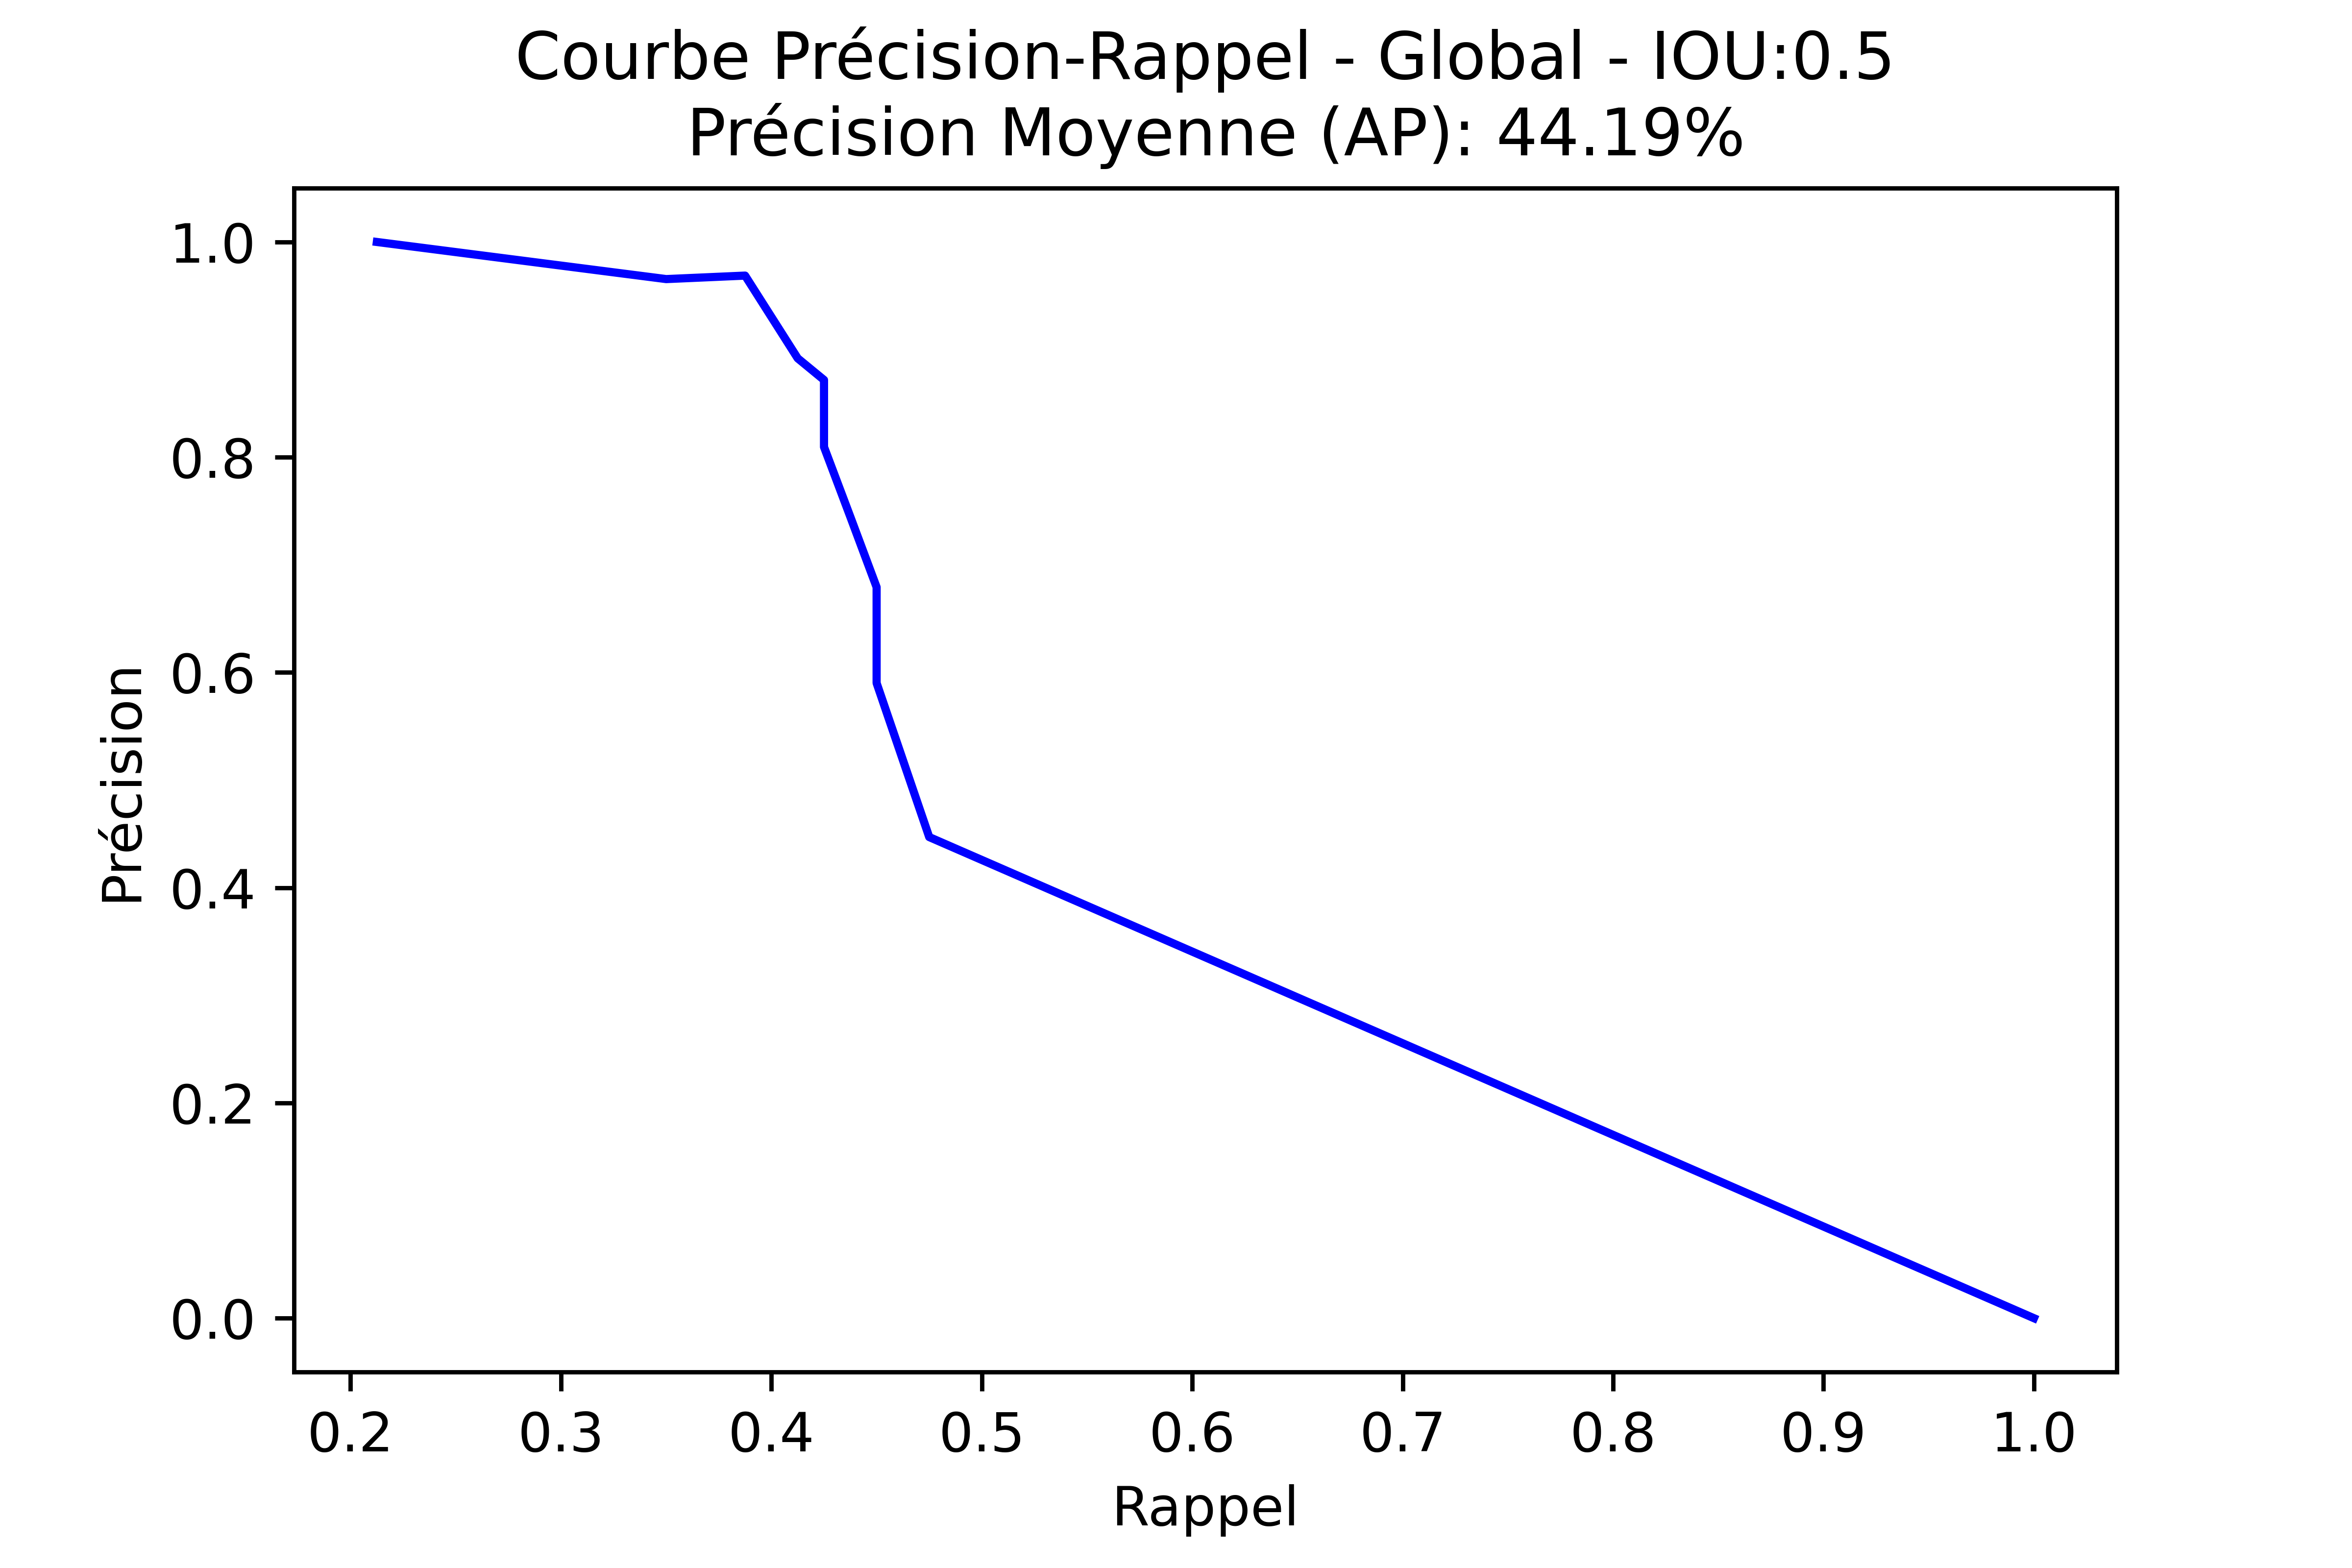
\includegraphics[height=10cm,width=17cm]{Chapitre3/yolov5_pr_global.png}
               \caption{YOLOv5: Courbe Précision-Rappel et Précision Moyenne de modéle.}
               \label{y4_pr}
               \end{figure}
     
     
     Le modèle réussit à détecter les URL écrites à l'aide de la police Arial de couleur noire avec $100\%$ de précision moyenne, l'épaisseur de la police n'affecte pas les résultats. 
     \begin{figure}[H]
               \centering
               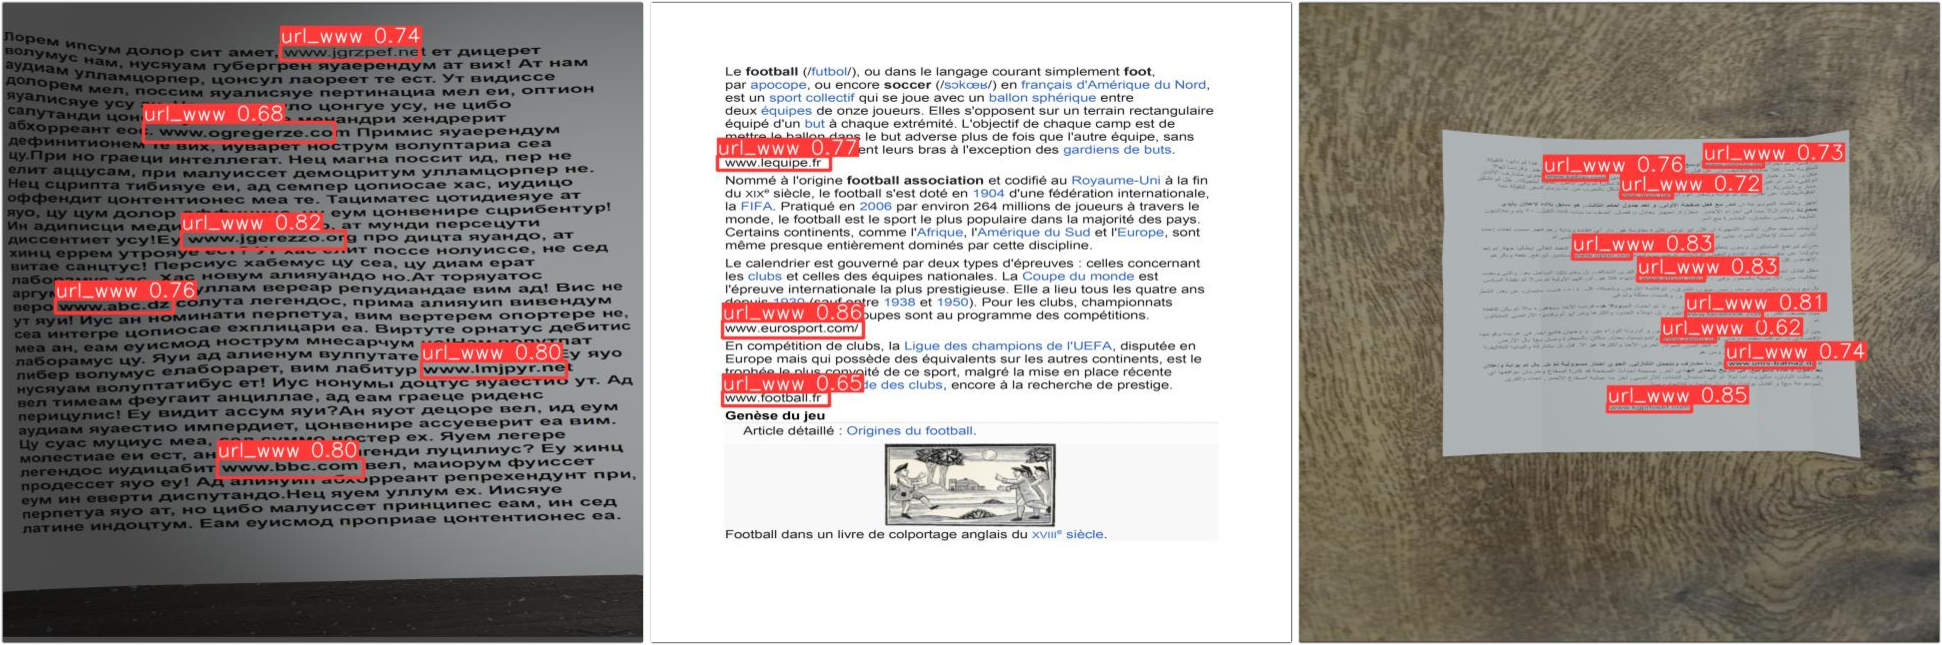
\includegraphics[height=10cm,width=17cm]{Chapitre3/y5_t1.png}
               \caption{YOLOv5 : Test des URL écrites en police Arial.}
               \label{y5_t1}
               \end{figure}

     Le modèle fait un excellent travail en détectant les URL écrites dans une police différente avec $88.05\%$ de précision moyenne.
     \begin{figure}[H]
               \centering
               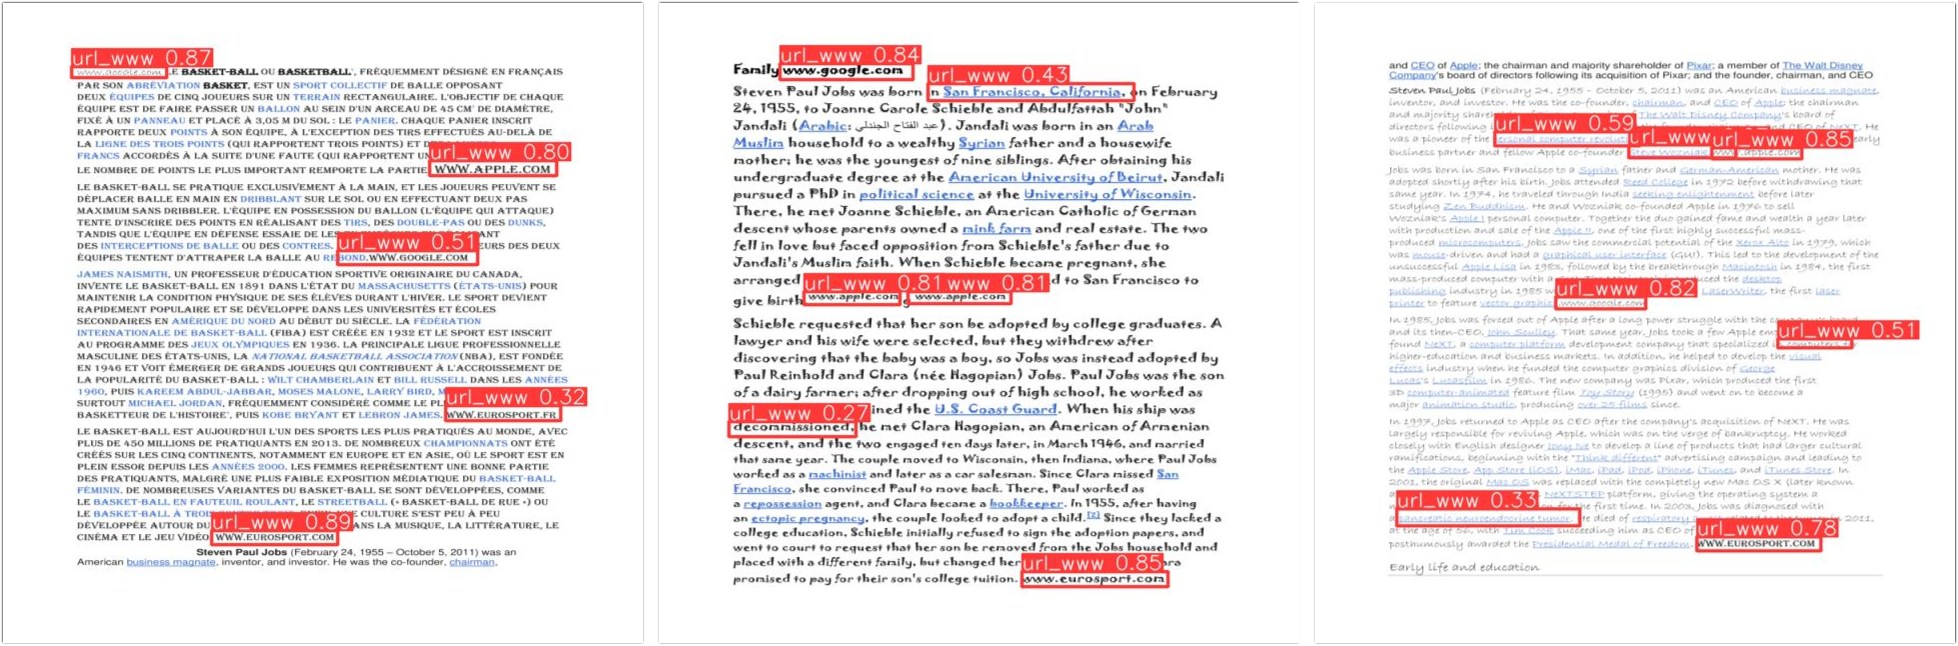
\includegraphics[height=10cm,width=17cm]{Chapitre3/y5_t2.png}
               \caption{YOLOv5: Test des URL écrites dans différentes polices.}
               \label{y5_t2}
               \end{figure}

     Pour les lettres d'URL colorées et les URL de couleur d'arrière-plan, le modèle ne parvient pas à les détecter correctement avec $27.27\%$ précision moyenne.
     \begin{figure}[H]
               \centering
               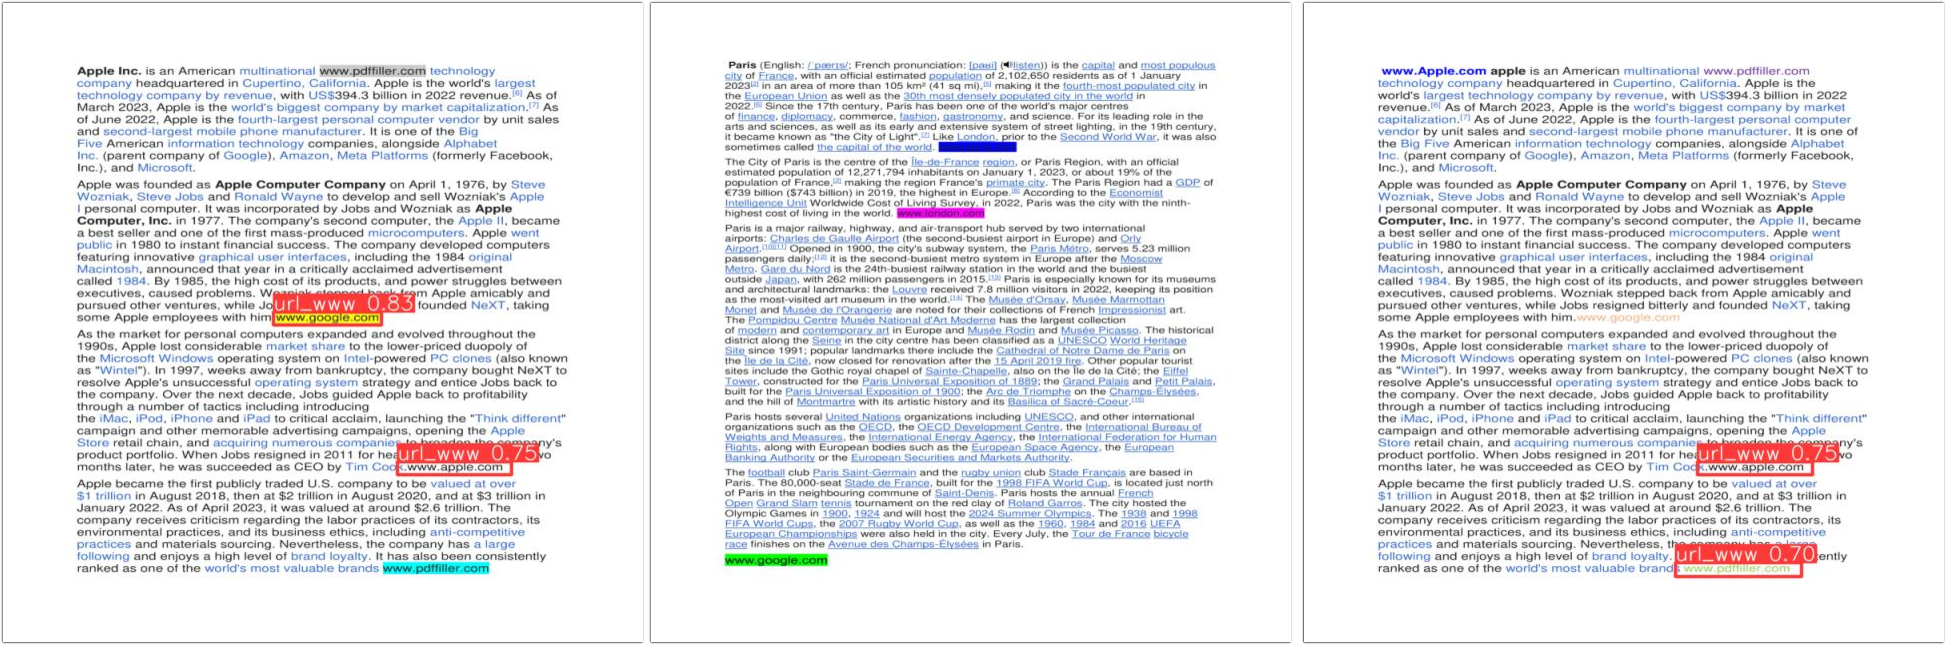
\includegraphics[height=10cm,width=17cm]{Chapitre3/y5_t3.png}
               \caption{YOLOv5 : test des URL écrites dans différentes couleurs.}
               \label{y5_t3}
               \end{figure}

     Pour les transformations, la mise à l'échelle n'affecte pas les résultats, par contre, les rotations affectent grandement la précision des modèles. Dans les rotations à $90 °$, le modèle échoue totalement à détecter les URL avec $0\%$ de précision, mais à $180 °$, le modèle détecte les URL correctement, comme si la rotation ne s'était jamais produite.
     \begin{figure}[H]
               \centering
               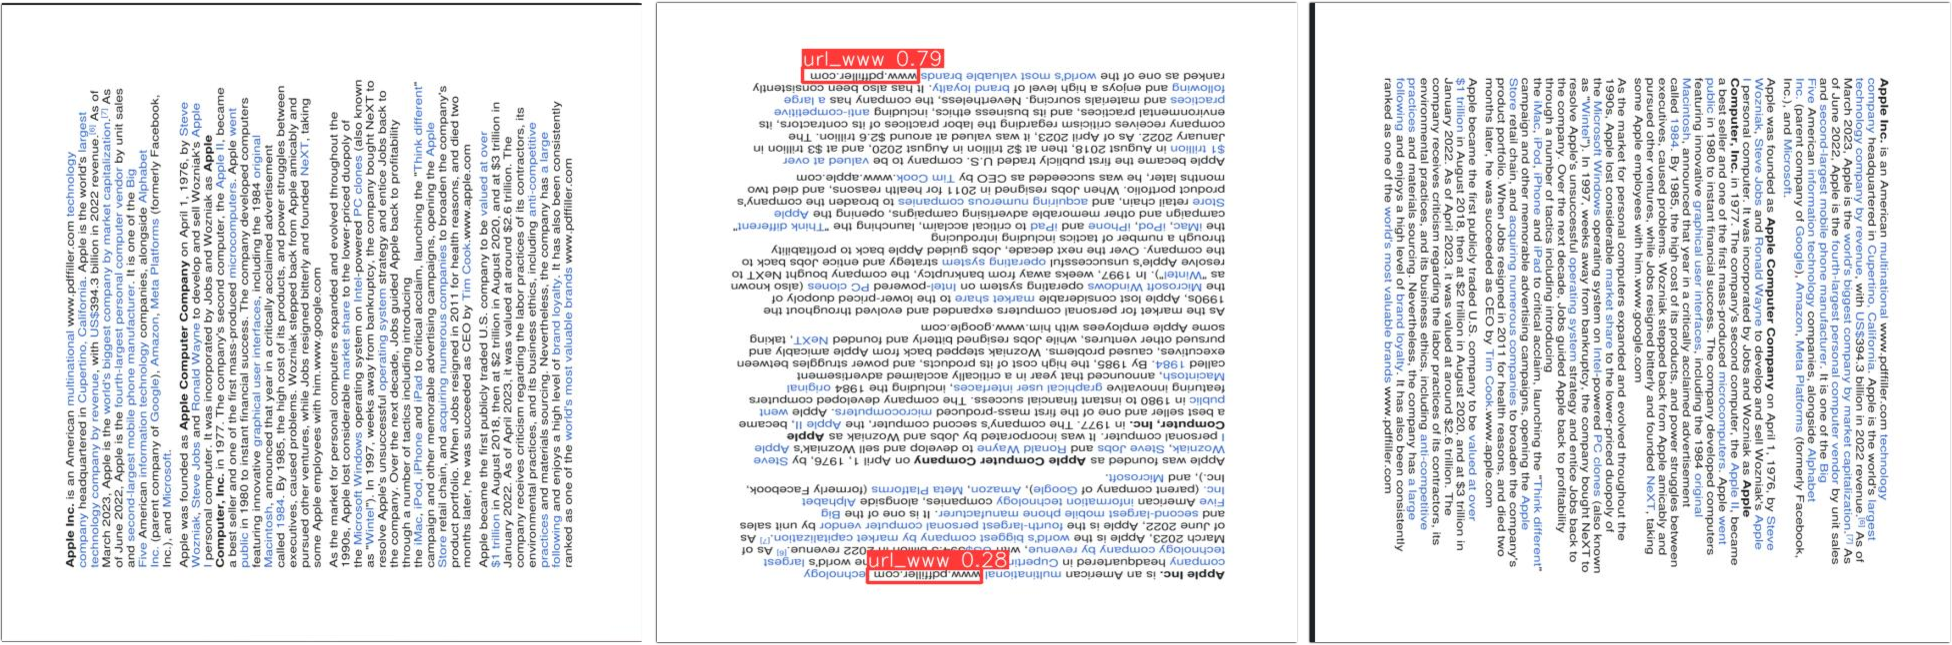
\includegraphics[height=10cm,width=17cm]{Chapitre3/y5_t4.png}
               \caption{YOLOv5: test des URL écrites dans différentes rotations.}
               \label{y5_t4}
               \end{figure}
     
     Dans le cas d'URL avec le protocole de préfixe https, le modèle ne parvient pas à donner des prédictions précises avec $13.6\%$ précision moyenne
     \begin{figure}[H]
               \centering
               \includegraphics[height=9cm,width=17cm]{Chapitre3/yolov5_https.png}
               \caption{YOLOv5 : test des URL écrites avec prefixe protocol HTTPS.}
               \label{y5_https}
               \end{figure}
     

     Enfin, pour les URL manuscrites, le modèle échoue totalement à effectuer une détection correcte. Cependant, il a détecté la première partie de l'URL $www.$ mais ne parvient pas à détecter l'intégralité de l'URL.
     \begin{figure}[H]
               \centering
               \includegraphics[height=11cm,width=12cm]{Chapitre3/y5_t5.jpg}
               \caption{YOLOv5 : Test des URL écrites en manuscrit.}
               \label{y5_t5}
               \end{figure}

     \paragraph{Conclusion:} La police et l'épaisseur des lettres n'affectent pas la précision du modèle. Cependant, les lettres colorées et l'arrière-plan des URL affectent la précision du modèle, en plus de cela, une rotation de 90 degrés affecte également la précision. Dans le manuscrit, le modèle échoue totalement à détecter une URL. De plus, le modèle vu détecte également les faux objets contenant des points ou des virgules.
     La solution consiste à incrémenter l'amélioration de l'ensemble de données pour qu'il contienne des exemples plus généralisés qui incluent les problèmes précédents.

\section{Conclusion Géneral}